\documentclass[12pt,a4paper]{article}
% Encoding
%\usepackage[utf8]{inputenc}
%\usepackage[T1]{fontenc}
% Deutsches Sprachpaket
\usepackage[ngerman]{babel}
% Font: Helvetica
\usepackage{helvet}
\renewcommand{\familydefault}{\sfdefault}
\usepackage{amsmath}
\usepackage{amsfonts}
\usepackage{amssymb}
\usepackage{graphicx}
\usepackage[left=3cm,right=2.5cm,top=2.5cm,bottom=2.5cm]{geometry}
\usepackage[headsepline,footsepline]{scrlayer-scrpage}
\usepackage{microtype}
\usepackage{pdfpages}
\usepackage{color}
\usepackage{listings}
\usepackage{xcolor}
% Farben für Codehighlighting
\definecolor{codegreen}{rgb}{0,0.6,0}
\definecolor{codegray}{rgb}{0.5,0.5,0.5}
\definecolor{codepurple}{rgb}{0.58,0,0.82}
\definecolor{backcolour}{rgb}{0.95,0.95,0.92}
\usepackage[hyphens]{url}
\usepackage[official]{eurosym}
\usepackage{array}
\usepackage{subcaption}
\usepackage{tabularx}
\usepackage{lastpage}
\usepackage[colorlinks=true,urlcolor=blue,linkcolor=black]{hyperref}
\hyphenpenalty=9999
\exhyphenpenalty=9999
\setlength{\headheight}{25pt}
\pagestyle{scrheadings}
\clearpairofpagestyles
\clearmainofpairofpagestyles
\clearplainofpairofpagestyles
\author{Felix Kuschel
	\and Manuel Starz}
\title{Entwicklung einer Smart Home Zentrale auf Basis eines RaspberryPI}
% Kopfzeile
\ihead{\includegraphics[width=0.2\textwidth]{pdf/its_logo.pdf}}
\chead{}
\ohead{\textsc{Seite \pagemark\:von \pageref{LastPage}}}
% Fußzeile
\ifoot{\textsc{FTI2 2020/2021}}
\cfoot{}
% Achtung, Muss 2 mal comilieren, sonst Fehler bei maximalen Seitenanzahl.
\ofoot{\textsc{Kuschel \& Starz}} 
\date{-}
\definecolor{quotetext}{rgb}{.35,.35,.35} %{1,.64,0}
% Codehighlighting stylesheet
\lstdefinestyle{mystyle}{
    backgroundcolor=\color{backcolour},   
    commentstyle=\color{codegreen},
    keywordstyle=\color{magenta},
    numberstyle=\tiny\color{codegray},
    stringstyle=\color{codepurple},
    basicstyle=\ttfamily\footnotesize,
    breakatwhitespace=false,         
    breaklines=true,                 
    captionpos=b,                    
    keepspaces=true,                 
    numbers=left,                    
    numbersep=5pt,                  
    showspaces=false,                
    showstringspaces=false,
    showtabs=false,                  
    tabsize=2
}
\lstset{style=mystyle}
\begin{document}
	% Titelseite
	% Basierend auf https://de.wikibooks.org/wiki/LaTeX/_Eine_Titelseite_erstellen
\begin{titlepage}
	\centering
	\includegraphics[width=0.5\textwidth]{pdf/its_logo.pdf}\par\vspace{1cm}
	% {\scshape\LARGE it.schule stuttgart \par}
	\vspace{1cm}
	{\scshape\Large Technikerarbeit\par}
	\vspace{1.5cm}
	{\huge\bfseries\scshape Entwicklung einer Smart Home Zentrale auf Basis eines Raspberry PI\par}
	\vspace{2cm}
	{\Large Felix \textsc{Kuschel} \& Manuel \textsc{Starz}\par}
	\vfill
	Betreut durch\par
	~Matthias \textsc{Kohler}

	\vfill

	% Bottom of the page
	{\large \today\par}
\end{titlepage}
	% Inhaltsverzeichnis
	\tableofcontents
	\newpage
	% Erklärung
	\section*{Erklärung}\label{erklaerung}
Wir versichern, dass die vorliegende Abschlussarbeit von uns selbstständig angefertigt und nur die angegebenen Hilfsmittel benutzt wurden. An Stellen, die dem Wortlaut oder dem Sinne nach anderen Werken entnommen sind, haben wir dies durch die Angabe der Quellen kenntlich gemacht.
\vspace{2cm}	
\\
\noindent\rule{7cm}{.4pt}\hfill\rule{7cm}{.4pt}\par
\noindent Datum, Ort \hfill Felix Kuschel
\vspace{2cm}	
\\
\noindent\rule{7cm}{.4pt}\hfill\rule{7cm}{.4pt}\par
\noindent Datum, Ort \hfill Manuel Starz
\newpage
	% Vorwort
 	\section{Vorwort}
\subsection{Einleitung}
Bei dieser Ausarbeitung handelt es sich um die Abschlussarbeit zur Weiterbildung zum staatlich geprüften Techniker in der Fachrichtung Informationstechnik. Diese Arbeit basiert auf dem in den zwei Jahren erlernten Stoffs sowie selbst erarbeiteten Kenntnissen und dient zur Feststellung des Erreichen des Fortbildungsziels.
\subsection{Projektrahmen}\label{vw_projektrahmen}
Das Projekt zur Erstellung einer Smart Home Zentrale wurde von uns, Felix Kuschel und Manuel Starz, durchgeführt. 
Der Projektzeitraum war vom 1. September 2020 bis zum 30. März 2021 angesetzt. 
Es stand zur Umsetzung des Projekts ein unterrichtsfreier Tag pro Woche zur Verfügung.\\
\noindent Des Weiteren wurden die in dem Zeitraum zur Verfügung stehenden Ferien zur Umsetzung des Projekts genutzt. Die Projektbetreuung erfolgt seitens der Schule durch Herr Matthias Kohler. 
Da das Projekt nicht in Zusammenarbeit mit einem Unternehmen durchgeführt wird, gibt es keine weiteren Betreuer. 
Die Materialkosten für die im Projekt genutzte Hardware wurde von uns selbst getragen.
Der im Lastenheft (vgl. Anhang \ref{ah_lastenheft}: \nameref{ah_lastenheft}) erwähnte Verein ,,Smart Home e.V.'' ist ein fiktiver Verein und dient lediglich als Platzhalter.
\subsection{Aufgabenstellung}\label{vw_aufgabenstellung}
Das Projekt ist aus dem Zusammenschluss der Abschlussarbeitsideen von uns, Felix Kuschel und Manuel Starz, entstanden und wurde in Rücksprache mit dem betreuenden Lehrer entwickelt.\par
\noindent Durch die große Verfügbarkeit von Smart Home Geräten und den zahlreichen Standards der Anbieter entschlossen wir uns, eine einfache und leicht zu replizierende Lösung zu entwickeln, mit der Smart Home Geräte mehrerer Hersteller miteinander verknüpft werden können und so die Notwendigkeit entfällt verschiedene sogenannte Hubs zu müssen.\par
\noindent Das Gerät soll darüber hinaus noch über einen Touchscreen steuerbar sein und die Parameter aller verbundenen Smart Home Geräte anzeigen.
Dies umfasst unter anderem den Status von Leuchtmitteln, die Parameter von Thermostaten, sowie den Zustand von Tür- und Fensterkontakten. 
Die genaue Aufgabenstellung kann dem abgegebenen Lastenheft im Anhang (\ref{ah_lastenheft}: \nameref{ah_lastenheft} entnommen werden.
\subsection{Zusatzinformationen}\label{vw_zusatzinformationen}
Die Rohdaten des Projekts wurden der Einfachheit halber in einem GIT-Projekt zusammengefasst.
Dadurch koönnen wir unabhängig voneinander an dem Projekt und der Dokumentation arbeiten.
\noindent Der Link zu dem Projekt lautet:\\
\url{https://github.com/Pharias/TAR}\par
\noindent Ursprünglich war dafür die Verwendung des schulinternen GIT geplant.
Dieses stand zum Zeitpunkt der Erstellung der Dokumentation allerdings nicht zur Verfügung\footnote{War lt. Herr Kohler nicht verfügbar aufgrund von Sicherheitsrisiken}, weshalb GITHub genutzt wurde.

\subsection{Definition Smart Home Zentrale}\label{vw_definition}
 	\begin{figure}[ht!]
 		\centering
 		\begin{subfigure}[t]{0.3\linewidth}
 			\centering
 			\includegraphics[width=0.9\textwidth]{img/alexa_echo_show8.jpg}
 			\caption[Amazon Alexa Echo Show 8]{Amazon Alexa Echo Show 8}
 			\label{fig:alexa-echo-show8}
 		\end{subfigure}
 		\hfill
 		\begin{subfigure}[t]{0.3\linewidth}
 			\centering
 			\includegraphics[width=0.9\textwidth]{img/google_nest_hub.png}
 			\caption[Google Nest Hub]{Google Nest Hub}
 			\label{fig:google-nest-hub}
 		\end{subfigure}
 		\hfill
 		\begin{subfigure}[t]{0.3\linewidth}
 			\centering
 			\includegraphics[width=0.9\textwidth]{img/glancr_smart_mirror.jpeg}
 			\caption[Glancr Smart Mirror]{Glancr Smart Mirror}
 			\label{fig:glancr-smart-mirror}
 		\end{subfigure}
 		\caption[Beispiele für Smart Home Zentralen]{Smart Home Zentralen}
 		\label{fig:smart-home-zentralen}
 	\end{figure}
\noindent Smart Home Zentralen, auch Smart Hubs oder Smart Mirrors genannt, sind Geräte, die als zentraler Knotenpunkt in einem Smart Home Netzwerk sitzen und dort Informationen verarbeiten, weiterleiten und darstellen können.\par
\noindent Diese Geräte werden von den meisten Herstellern mit und ohne Bildschirm geliefert, um entweder ein neues Smart Home aufzubauen oder ein bestehendes Smart Home zu erweitern. 
 	\begin{quote}
 		\color{quotetext}
 		Bei einem Smart-Home-Hub handelt es sich um eine schlaue Zentrale, durch die all deine intelligenten Geräte miteinander vernetzt werden – und dadurch erst wirklich ihren gesamten Leistungsumfang ausschöpfen.\footnote{Li (2017): Was ist ein Smart-Home-Hub? Alles über die intelligente Zentrale}
 	\end{quote}
\noindent Als Smart Home Zentrale können auch Software-Lösungen gezählt werden, die mit den im Netz befindlichen Smart Hubs kommunizieren und die Informationen mit Hilfe eines Web-Interfaces oder einer Smartphone-Anbindung darstellen und steuern können. 
Beispiele hierfür sind homeassistant.io, openHAB und Google Home.\par
% WARUM WILL DAS NIT ANGEZEIGT WERDEN!!!
\begin{figure}[h!tb]
 	\centering
 	\begin{subfigure}[b]{0.3\linewidth}
 		\centering
 		\includegraphics[width=0.7\textwidth]{img/home-assistant-io_logo.png}
 		\caption[Home Assistant Logo]{Home Assistant}
 		\label{fig:hassio-logo}
 	\end{subfigure}
 	\hfill
 	\begin{subfigure}[b]{0.3\linewidth}
 		\centering
 		\includegraphics[width=0.7\textwidth]{img/google-cast_logo.png}
 		\caption[Google Home Logo]{Google Home}
 		\label{fig:google-home-logo}
 	\end{subfigure}
 	\hfill
 	\begin{subfigure}[b]{0.3\linewidth}
 		\centering
 		\includegraphics[width=0.7\textwidth]{img/openhab_logo.png}
 		\caption[openHAB Logo]{openHAB}
 		\label{fig:openhab-logo}
 	\end{subfigure}
 	\caption[Beispiele für Smart Home Software]{Smart Home Software}
 	\label{fig:software-logos}
\end{figure}
\newpage
 	% Zielsetzung
	\section{Zielsetzung}\label{zielsetzung}
Als Ziel für das Projekt war ein funktionsfähiges Smart Home Hub mit Zigbee-Anbindung auf Basis eines Raspberry Pi 4 geplant. 
Das Smart Home Hub in seiner Grundfunktion soll in der Lage sein, die mit ihm verbundenen Geräte über den Zigbee-Standard anzusteuern.
Zusätzlich sollte die Möglichkeit einer Erweiterung mit einem Sprachassistenten möglich sein.\par
% Konzeption
\subsection{Konzeption}\label{zs_konzeption}
Zu Beginn des Projekts haben wir Nachforschung angestellt und uns bereits vorhandene Open-Source-Lösungen im Bereich Smart Home näher angeschaut.
Dabei sind wir neben dem Smart Mirror GLANCR auch auf die Gesamtlösungen homeassistant.io sowie openHAB gestoßen. 
In Folge dessen haben wir ein Grundkonzept in unserem Lastenheft zusammengefasst und dieses in Absprache mit unserem Betreuungslehrer, Herr Kohler, ausgearbeitet und abgegeben.\par
\noindent Dann konnten wir uns an die Beschaffung der unserer Meinung nach notwendigen Komponenten für das Projekt machen.

% Anforderungen und gewünschte Features
\subsection{Anforderungen und gewünschte Features}\label{zs_anforderungen}
Die Anforderungen an das Projekt lauteten demnach wie folgt:
\begin{itemize}
	\item Anbindung von ZigBee-fähigen Endgeräten
	\item Steuerung der angebundenen Endgeräte
	\item Übermittlung der Zustände der angebundenen Geräte an z.B. ein Smartphone
\end{itemize}
Diese Anforderungen lassen sich mit einem Raspberry Pi und einem Zigbee-USB-Stick realisieren. Darüber hinaus waren von unserer Seite noch folgende Features gewünscht:
\begin{itemize}
	\item Ein- und Ausgabe über einen Touch-Bildschirm
	\item Einbindung eines Sprachassistenten zur Steuerung der eingebundenen Endgeräte
\end{itemize}
Nach Fortschritt des Projekts kam bei einer Rücksprache mit unserem Projektbetreuer die Idee auf, einen Raspberry Pi Hat speziell für das Projekt zu entwickeln. Dieser sollte die Hardware des Projekts falls möglich auf einer Platine vereinen, die dann auf den Raspberry Pi aufgesteckt werden konnte.\par
Diese Erweiterungsplatine sollte folgende Eigenschaften besitzen:
\begin{itemize}
	\item ZigBee-Controller und Antenne
	\item NFC-Controller und Antenne
	\item RGB-LED zur Statusanzeige
	\item Anschluss für Lüfter
	\item Sensoren für:
	\begin{itemize}
		 \item Luftfeuchtigkeit
		 \item Temperatur
		 \item Luftdruck
	\end{itemize}
	\item Pins zum Anschluss an Versuchsaufbau für Laborgebrauch
\end{itemize}
Die Erweiterungsplatine wurde aber wie zuvor aufgrund der aktuellen Pandemie-Situation und den damit verbundenen Beschaffungsschwierigkeiten verworfen.
Darauf wurde dann klar, dass eine Erstellung eines Installationsskripts für den Raspberry Pi eine sinnvolle Ergänzung der Projektarbeit wäre. Zusätzlich haben wir ein Gehäuse für die Hardware geplant, um das Endprodukt so wertiger gestalten zu können.
% Erweiterungsmöglichkeiten
\subsection{Erweiterungsmöglichkeiten}\label{zs_erweiterung}
Als eine Erweiterung des Projekts ist ein sogenannter Raspberry Pi HAT, eine aufsteckbare Erweiterung für den Raspberry Pi geplant.
% Nach Fortschritt des Projekts kam bei einer Rücksprache mit unserem Projektbetreuer die Idee auf, einen Raspberry Pi HAT speziell für das Projekt zu entwickeln. 
Die Idee dazu entstand in Rücksprache mit unserem Projektbetreuer, der den HAT darüber hinaus als Unterrichtsmaterial im Laborunterricht einsetzten wollte.
Dieser sollte die Hardware des Projekts, falls möglich auf einer Platine vereinen.\par
\noindent Der HAT sollte folgende Bauteile enthalten:
\begin{itemize}
	\item ZigBee-Controller und Antenne
	\item NFC-Controller und Antenne
	\item RGB-LED zur Statusanzeige
	\item Anschluss für Lüfter
	\item Sensoren für:
	\begin{itemize}
		 \item Luftfeuchtigkeit
		 \item Temperatur
		 \item Luftdruck
	\end{itemize}
	\item Pins zum Anschluss an Versuchsaufbau für Laborgebrauch in der Schule
\end{itemize}
Der HAT wurde aber aufgrund der aktuellen Pandemie-Situation und den damit verbundenen Liefer- und Zollschwierigkeiten verworfen.
Die Planung des HAT ist daher nicht vollständig, kann aber bei Bedarf ergänzt werden (vgl. Abschnitt \ref{hw_hat}: \nameref{hw_hat}).
\newpage
	% Herangehensweise
	\section{Herangehensweise}\label{herangehensweise}
Nach Festlegung der Anforderungen haben wir uns dann an die Beschaffung und der benötigten Materialien und die Einrichtung der Hard- und Software gemacht. 
Hierfür haben wir zum Teil bereits vorhandene Hardware, z.B. den Raspberry Pi 4 mit weiteren Komponenten wie dem Touch-Bildschirm und den Lautsprechern sowie dem Mikrofon ergänzt. 
Damit ist die Umsetzung des Projekts in zwei Teile geteilt:
% Hardware
\subsection{Hardware}\label{hgw_hardware}
Bei der Entwicklung der Hardware haben wir für unser Projekt intern einige Rahmenbedinungen festgelegt:
\begin{itemize}
	\item Das Projekt sollte nach Möglichkeit von durchschnittlichen Bastlern durchgeführt werden
	\item Zur Fertigstellung des Projekts sollte mit Handelsüblichen Bastler Werkzeugen möglich sein
	\item Die Grundplattform sollte der 2020 herausgebrachte Raspberry Pi 4 8GB sein\footnote{Wikipedia: Raspberry Pi - Generations}
	\item Das Gerät sollte möglichst von vielen Herstellern vertriebenen Zigbee-Endgeräte verwalten können.
\end{itemize}
\noindent Die Beschaffung der Teile lief dank Online-Versandhandel relativ problemlos. 
Beim Zusammenbau haben wir den Prototyp lediglich mit dem Bildschirm, dem Pi und dem Zigbee-USB-Stick aufgebaut (vgl. Abschnitt \ref{hw_prototype}: \nameref{hw_prototype}). 
Die beiden Standfüße stammen vom Hersteller des Bildschirms Sunfounder \footnote{Sunfounder: 10.1 Inch Touch Screen for Raspberry Pi(NEW) - 3D-printed Touch Screen Support}.
Diese haben wir aus PETG auf dem Ender 3 gedruckt. 
Anschließend haben wir die Softwareseite des Projekts bearbeitet (vgl. Abschnitt \ref{hgw_software}: \nameref{hgw_software} \& Kapitel \ref{software}: \nameref{software}).\par
\noindent Nachdem der Prototyp soweit funktionsfähig war, haben wir uns daran gemacht, das Präsentationsmodell zu entwerfen. 
Dabei ging es uns vornehmlich um die Unterbringung der geplanten Komponenten in einem simplen Gehäuse. 
Hierfür waren einige Verlängerungskabel nötig, um Stromzufuhr, Netzwerk und die Antenne des Zigbee-Sticks nach außen zu leiten (vgl. Abschnitt \ref{hw_case_modellentwicklung}: \nameref{hw_case_modellentwicklung} \& Abschnitt \ref{ku_produkt}: \nameref{ku_produkt}). \\
\noindent Das Gehäuse wurde dann nach dem Druck mit dem Bildschirm verklebt und die einzelnen Komponenten verbaut (vgl. Abschnitt \ref{hw_case_herstellung}: \nameref{hw_case_herstellung}). 
Nachdem das Gerät soweit fertig war, haben wir einen Versuchsaufbau zur Präsentation aufgebaut, der die Funktionsweise des Geräts in einem ,,typischen'' Heimnetzwerk darstellen soll (vgl. Abschnitt \ref{hw_testaufbau}: \nameref{hw_testaufbau}).\\
\noindent Näheres zur Herangehensweise im Kapitel \ref{hardware}: \nameref{hardware}.
% Software
\subsection{Software}\label{hgw_software}
\subsubsection{Home Assistant}\label{hwg_software_homeassistant}
Auf der Softwareseite haben wir uns bereits verfügbare Lösungen für Smart Home Zentralen angeschaut. 
Ursprünglich war unser Plan, eine eigene Softwarelösung mit Web-Interface oder einer App-Anbindung für Smartphones selbst zu programmieren.\\
\noindent Diese Idee haben wir nach kurzer Zeit aber wieder verworfen, da dieser Markt bereits mehr als gesättigt ist mit kostenlosen als auch kostenpflichtigen Lösungen. 
Von den kostenlosen und quelloffenen Lösungen war für uns Home Assistant am interessantesten, vor allem wegen der breiten Menge an Addons und der unserer Meinung nach recht ansprechenden Web-Oberfläche.
Home Assistant verfügt über drei grundlegende Möglichkeiten, installiert zu werden:
\begin{itemize}
    \item Als eigenes Betriebssystem-Image (Home Assistant Operating System)
    \item Als Docker Container
    \item Als Programm auf einem Server
\end{itemize}
Unabhängig von der Installationsart wird der Home Assistant in zwei Versionen angeboten:
\begin{itemize}
    \item Als Core Version
    \item Als Supervised Version
\end{itemize}
Die Core Version ist die grundlegende Version des Home Assistants während die Supervised Version ein Addon-Repository integriert hat. \footnote{siehe \url{https://www.home-assistant.io/installation/}}\\
\noindent Darüber hinaus vertreibt Home Assistant auch noch eine fertige Out-of-the-Box-Lösung namens Home Assistant Blue\footnote{siehe \url{https://www.home-assistant.io/blue}} für 140\$, allerdings gibt es nur wenige Länder, in denen das Gerät verfügbar ist und es besitzt anders als unsere Lösung keinen Bildschirm.\\
\noindent Für unsere Anwendung war das eigene Betriebssystem-Image nicht verwendbar, da sich auf dem System keine grafische Oberfläche nachinstallieren ließ. 
Deshalb haben wir uns zuerst auf die Programm-Variante des Home Assistants entschieden.\\
\noindent Allerdings gab es bei der Installation der Supervised Version auf unterschiedlichen Pi-Versionen Probleme und die Core-Version war für unsere Zwecke ungeeignet, da hier der Arbeitsaufwand für die die Integration von zusätzlichen Komponenten und Systemerweiterungen für die Zielgruppe des Projekts zu komplex ist. 
Außerdem hat sich während unserer Testphase gezeigt das die Verknüpfung von Home Assistant Core, Mosquitto Broker sowie Zigbee2MQTT zu nicht dauerhaft reproduzierbaren Erfolgen führt und sich deshalb leider nicht wie von uns geplant automatisieren lässt. 
Deshalb haben wir uns für die Container-Variante mit Docker entschieden. 
Das Installationsskript (vgl. \ref{ah_skript}: \nameref{ah_skript}) installiert die benötigten Programme und übernimmt die Grundeinrichtung des Homeassistants bis zum Punkt an dem die Einrichtung in der Weboberfläche durch den Nutzer stattfindet.\\
\noindent Um neben dem Skript noch eine weitere Art der Einrichtungsmöglichkeit anzubieten zu können, haben wir von den SD-Karten nach Ablauf des Installationsskripts ein Backup-Image erstellt und dieses entsprechend der beiden in Verwendung befindlichen Raspberry Pi Versionen\footnote{Raspberry Pi B Version 3 und Version 4(8GB)} erstellt.
Der Benutzer und das Passwort entsprechen bei den Images den standardmäßig in Raspberry Pi OS hinterlegten Nutzern und sollten beim booten sicherheitshalber geändert werden\\
\noindent Näheres zur Herangehensweise im Kapitel \ref{software}: \nameref{software}.
\subsubsection{MQTT und Zigbee2MQTT}\label{hwg_software_mqtt_zibee2mqtt}
Um die von uns Angestrebte Steuerung und Integration von Zigbee Leuchtmitteln und Geräten zu ermöglichen, benötigen wir den Übertragungsstandard MQTT und die Möglichkeit die Zigbee Daten über diesen an Home Assistant weiter zu reichen. 
Wir haben uns schon sehr früh auf einen MQTT broker und die Anwendung für Verarbeitung des Zigbee-Protokolls entschieden.
\begin{itemize}
    \item Mosquitto broker (Opensource MQTT broker)
    \item Zigbee2MQTT als Zigbee Schnittstelle
\end{itemize}
\noindent Beschreibung Mosquitto broker
\begin{quote}
    \color{quotetext}
 	    Eclipse Mosquitto ist ein Open Source (EPL/EDL lizenziert) Message Broker, der das MQTT-Protokoll in den Versionen 5.0, 3.1.1 und 3.1 implementiert. Mosquitto ist leichtgewichtig und eignet sich für den Einsatz auf allen Geräten, von stromsparenden Einplatinencomputern bis hin zu kompletten Servern.

        Das MQTT-Protokoll bietet eine leichtgewichtige Methode zur Durchführung von Messaging unter Verwendung eines Publish/Subscribe-Modells. Dadurch ist es für das Internet der Dinge geeignet, z. B. für Sensoren mit geringem Stromverbrauch oder mobile Geräte wie Telefone, eingebettete Computer oder Mikrocontroller.

        Das Mosquitto-Projekt bietet auch eine C-Bibliothek zur Implementierung von MQTT-Clients und die sehr beliebten mosquitto-pub und mosquitto-sub Kommandozeilen-MQTT-Clients.\footnote{mosquitto.org (Übersetzt mit DeepL): \url{https://mosquitto.org/}}
\end{quote}
\noindent Beschreibung Zigbee2MQTT
\begin{quote}
    \color{quotetext}
 		Zigbee2MQTT besteht aus drei Modulen, die jeweils in einem eigenen Github-Projekt entwickelt wurden. Beginnend bei der Hardware (Adapter) und aufsteigend; zigbee-herdsman verbindet sich mit Ihrem Zigbee-Adapter und stellt eine API für die höheren Ebenen des Stacks zur Verfügung. Für z.B. Texas Instruments Hardware verwendet zigbee-herdsman die TI zStack Monitoring und Test API, um mit dem Adapter zu kommunizieren. Zigbee-herdsman übernimmt die zentrale Zigbee-Kommunikation. Das Modul zigbee-herdsman-converters übernimmt das Mapping von einzelnen Gerätemodellen auf die von ihnen unterstützten Zigbee-Cluster. Zigbee-Cluster sind die Schichten des Zigbee-Protokolls, die über dem Basisprotokoll liegen und z. B. definieren, wie Lampen, Sensoren und Schalter über das Zigbee-Netzwerk miteinander kommunizieren. Schließlich steuert das Zigbee2MQTT-Modul zigbee-herdsman und bildet die Zigbee-Nachrichten auf MQTT-Nachrichten ab. Zigbee2MQTT behält auch den Status des Systems im Auge. Es verwendet eine database.db-Datei, um diesen Zustand zu speichern; eine Textdatei mit einer JSON-Datenbank der angeschlossenen Geräte und ihrer Fähigkeiten.\footnote{github.com (Übersetzt mit DeepL): \url{https://github.com/koenkk/zigbee2mqtt}}
\end{quote}
\newpage
	% Zeitplan
	\section{Zeitplan}\label{zeitplan}
\begin{figure}[ht!]
	
\includegraphics[width=1\textwidth]{img/TAR_FKMS_20202021.png}
	\caption[gantt-Diagramm des Projektablaufs]{gantt-Diagramm des Projektablaufs}
 	\label{fig:gantt-diagramm}
\end{figure}
\newpage
	% Komplettübersicht
	\section{Komplettübersicht}
% Das "fertige" Produkt
\subparagraph{Das ,,fertige`` Produkt}
\begin{figure}[h!t]
	\includegraphics[width=1\textwidth]{img/placeholder.png}
	\caption[Smart Home Zentrale]{Smart Home Zentrale}
	\label{fig:smart-home-zentrale}
\end{figure}
\newpage
% Kostenaufstellung
\subsection{Kostenaufstellung}\label{ku_kosten}
Im Anschluss haben wir die Kosten des Projekts dargestellt (vgl. Tab \ref{tab:ku_gesamtkostenberechnung}: \nameref{tab:ku_gesamtkostenberechnung}\par
% Beschaffungskosten
\subsubsection{Beschaffungskosten}\label{ku_kosten_beschaffung}
\begin{center}
\begin{table}[H]
    \begin{tabularx}{\textwidth}{|p{5.6cm}|p{1.2cm}|p{3.44cm}|p{3.5cm}|}
        \hline
 	    \textbf{Produkt} & \textbf{Menge} & \textbf{Kosten pro Stück}  & \textbf{Kosten insgesamt}\\
	    \hline
	    \hline
	    Raspberry Pi 4 Modell B 8 GB & 1 & 87,22 \euro{} & 87,22 \euro{} \\
	    \hline
	    SanDisk Extreme microSD 128 GB & 1 & 19,99 \euro{} & 19,99 \euro{} \\
	    \hline
	    SUNFOUNDER RPi 10.1'' Touch Display & 1 & 129,99 \euro{} & 129,99 \euro{} \\
	    \hline
	    Noctua NF-A4x10 5v & 1 & 12,90 \euro{} & 12,90 \euro{} \\
	    \hline
	    ITSTUFF CC2531 Zigbee USB-Stick & 1 & 14,90 \euro{} & 14,90 \euro{} \\
	    \hline
	    ITSTUFF Alu-Kühlkörper Set RPi 4 & 1 & 4,91 \euro{} & 4,91 \euro{} \\
	    \hline
	    Eightwood SMA Verlängerung & 1 & 7,99 \euro{} & 7,99 \euro{} \\ 
	    \hline
	    VCE 5,5 mm Stecker \& Buchse & 1 & 8,29 \euro{} & 8,29 \euro{} \\
	    \hline
	    dasFilament PTGE schwarz 1,75 mm & 0,52 & 24,95 \euro{}\footnote{Kosten der Spule (800 g).} & 11,61\euro{}\footnote{Kosten verwendetes Material für Gehäusedruck} \\
	    \hline
	    USB-Verlängerung & 1 & 9,99 \euro{} & 9,99 \euro{}\\
	    \hline
	    \hline
	    % hier noch die Kosten für das Zeug, das du gekauft hast, Felix. der Stick steht ja schon drin, aber weiß nicht ob der Preis passt...
	    %\hline
	    \textbf{Gesamtkosten} &  &  & \textbf{309,37 \euro{}} \\ % Kosten zusammenrechnen ;)
	    \hline
    \end{tabularx}
    \caption{Beschaffungskosten}
    \label{tab:ku_kostenberechnung}
\end{table}
\end{center}
\newpage
% Arbeitszzeit
\subsubsection{Arbeitszeit}\label{ku_kosten_zeit}
Gerechnet wird in Stunden, ein Arbeitstag hat 8 Stunden.
\begin{center}
\begin{table}[H]
    \begin{tabularx}{\textwidth}{|p{11.8cm}|p{2.8cm}|}
        \hline
 	    \textbf{Projektabschnitt} & \textbf{Dauer (in h)} \\
	    \hline
	    \hline
	    Recherche & 60 \\
	    \hline
	    Themenfindung & 6 \\
	    \hline
	    Anfertigung Lastenheft & 20 \\
	    \hline
	    Beschaffung Hardware & 4 \\
	    \hline
	    Entwicklung Prototyp & 40 \\
	    \hline
	    Konstruktion Gehäuse & 40 \\
	    \hline
	    Software Installation & 8 \\
	    \hline
	    Entwurf Skript & 80 \\
	    \hline
	    Erstellung Images & 4 \\
	    \hline
	    Entwurf Raspberry Pi HAT & 30 \\
	    \hline
	    Dokumentation & 80 \\
	    \hline
	    Funktionsprüfung & 20 \\
	    \hline
	    Präsentationsaufbau & 8 \\
	    \hline
	    \hline
	    \textbf{Gesamt} & \textbf{400} \\
	    \hline
    \end{tabularx}
    \caption{Erfassung der Arbeitszeiten}
    \label{tab:ku_arbeitszeiten}
\end{table}
\end{center}
\noindent Bei dem aktuell gültigen Mindestlohn von 9,50 \euro{} \footnote{Deutscher Gewerkschaftsbund (2021): Mindestlohn 2021/2022: Was ändert sich?} kommen wir so auf Arbeitskosten von 3800 \euro{}.
% Kosten 3D-Druck
\subsubsection{Kostenberechung für die 3D-Druckteile}\label{ku_kosten_druck}
\noindent Die Kosten lassen mit folgender Formel darstellen:\\
\[
K_{gesamt} =  (K_{Material/g} \cdot M_{Material}) +  (T_{Druck} \cdot  K_{kWh} \cdot V_{\emptyset/h})
\]
Die Kosten der 3D-Druckteile lassen sich in zwei Einzelpositionen aufteilen: Material und Energie.
Die Materialkosten lassen sich leicht erfassen, da wir die Kosten der Spule Filament mit 24,95 \euro{} und einem Gewicht von 800 g Filament auf der Spule gegeben haben.
So ergibt sich ein Preis von 0,03(12...)\euro{} ($K_{Material/g}$) pro Gramm verwendetem Filament.
Der Druck der Gehäuseteile verbrauchte 423 g Material ($M_{Material}$), das heißt, dass die Materialkosten sich auf 13,19 \euro{} belaufen.\par
\noindent Die Energiekosten zu berechnen ist etwas komplexer.
Der 3D-Drucker verbraucht circa 120 W pro Stunde($V_{\emptyset/h}$)\footnote{Robert (2019): Antwort auf Creality Ender 3 printer power consumption? - 3dprinting Stack Exchange}, was bei einem Strompreis von 0,31 \euro{} / kWh ($K_{kWh}$) bedeuten würde, dass wir pro Stunde etwa 0,0372 \euro{} Stromkosten haben. 
Bei einer Gesamtdruckzeit von 36 Stunden und 36 Minuten($T_{Druck}$) ergeben sich also Stromkosten von 1,37 \euro{}.\par
\noindent Addiert man nun die Kosten für Material und Energie, so ergibt sich ein Fertigungspreis von 12,98 \euro{} ($K_{gesamt}$). 
Dabei ist der Zeitaufwand für die Veredelung, also Schleifen und Lackieren, noch nicht mit einkalkuliert.\par
% Kosten Präsentationsaufbau
\subsubsection{Kosten Präsentationsboard}\label{ku_kosten_praesi}
\begin{center}
\begin{table}[H]
    \begin{tabularx}{\textwidth}{|p{5.6cm}|p{1.2cm}|p{3.44cm}|p{3.5cm}|}
        \hline
 	    \textbf{Produkt} & \textbf{Menge} & \textbf{Kosten pro Stück}  & \textbf{Kosten insgesamt}\\
	    \hline
	    \hline
	    OSB Platte & 1 & 11,22 \euro{} & 11,22 \euro{} \\
	    \hline
	    Kantholz & 4,2 m & 1,38 \euro{} & 2,76 \euro{} \\
	    \hline
	    Lampenfassung E27 Schwarz & 2 & 2,99 \euro{} & 5,98 \euro{} \\
	    \hline
	    Winkelverbinder Gleichschenklig & 4 & 4,99 \euro{} & 19,96 \euro{} \\
	    \hline
	    Konstruktionswinkel & 2 & 1,19 \euro{} & 2,38 \euro{} \\
	    \hline
	    Schrauben & 1 & 12,99 \euro{} & 12,99 \euro{} \\
	    \hline
	    Mantelleitung NYM-J 3 x 1,5 Grau 5 m & 1 & 4,99 \euro{} & 4,99 \euro{} \\ 
	    \hline
	    Abzweigkasten Aufputz & 3 & 1,59 \euro{} & 4,77 \euro{} \\
	    \hline
	    Schutzkontakt Flachstecker mit seitlicher Einführung & 1 & 1,69 \euro{}\ & 1,69\euro{} \\
	    \hline
	    Schutzkontakt Steckdose & 1 & 6,99 \euro{} & 6,99 \euro{} \\
	    \hline
	    König KNM-FTM10 Tablet Wandhalterung & 1 & 10,55 \euro{} & 10,55 \euro{} \\
	    \hline
	    Philips HUE Smart Plug & 1 & 29,99 \euro{} & 29,99 \euro{} \\
	    %\hline
	    \hline
	    \hline
	    \textbf{Gesamtkosten} &  &  & \textbf{113,27 \euro{}} \\ % Kosten zusammenrechnen ;)
	    \hline
    \end{tabularx}
    \caption{Kosten Präsentationsaufbau}
    \label{tab:ku_kostenpraesi}
\end{table}
\end{center}
% Gesamtkosten
\subsubsection{Gesamtkosten}\label{ku_kosten_gesamt}
\begin{center}
\begin{table}[H]
    \begin{tabularx}{\textwidth}{|p{9.9cm}|p{4.7cm}|}
        \hline
 	    \textbf{Position} & \textbf{Kosten} \\
 	    \hline
 	    \hline
 	    Materialkosten & 309,37 \euro{} \\
	    \hline
	    Stromkosten Druck & 1,37 \euro{} \\
	    \hline
	    Stundenlohn & 3800,00 \euro{} \\
	    \hline
	    Kosten Präsentationsboard & 113,27 \euro{} \\
	    \hline
	    \hline
	    \textbf{Gesamtkosten} & \textbf{4224,01 \euro{}} \\ % Kosten zusammenrechnen ;)
	    \hline
    \end{tabularx}
    \caption{Gesamtkostenberechnung}
    \label{tab:ku_gesamtkostenberechnung}
\end{table}
\end{center}


\newpage
	% Hardware
	\section{Hardware}\label{hardware}
% Raspberry Pi 4
\subsection{Raspberry Pi 4}\label{hw_raspberrypi}
Als Basis für die Smart Home Zentrale haben wir einen Raspberry Pi in der Version 4 mit 8 GB gewählt, um als von anderen Servern unabhängige Plattform zu agieren. 
Der Raspberry Pi 4 ist mit einem ARM Cortex-A72 Prozessor ausgestattet, der über 4 Kerne verfügt.
Darüber hinaus verfügt der Raspberry Pi 4 über einen Gigabit-Netzanschluss.
Darüber hinaus ist der Raspberry Pi in der Bastlerszene weit verbreitet und dient bei anspruchsvolleren Projekten als Kern\par
\begin{quote}
 		\color{quotetext}
 		Der Raspberry Pi hat sich seit der ersten Veröffentlichung Anfang 2012 weltweit schon millionenfach verkauft und erfreut sich immer noch größter Beliebtheit. Denn viele Raspberry Pi User haben nicht nur einen Einplatinen-Computer zu Hause, sondern teils 4-5 Stück.
Der eine fungiert als HD-Mediaplayer mit externer Festplatte für das heimische Kino oder als Internetradio mit Display, der nächste als Webcam-Server für die Kameraüberwachung mit Livestream auf das Handy, dann noch einer für die Hausautomatisierung wie bspw. die Heizungs- oder Lichtsteuerung und noch einer als einfacher WLAN-Druckerserver oder als Mini-Computer zum allgemeinen Surfen im Internet, um ein paar wenige Anwendungsszenarien zu nennen.
Sie merken, der kleine ,,Tausendsassa'' kann nicht nur viel, sondern ist zudem auch noch extrem günstig und eben das macht den Reiz aus. Lediglich den Hang zum Programmieren sollten Sie mitbringen und selbst nicht mal das, denn Sie können auch einfach nach Anleitung aus Foren oder Büchern nachprogrammieren, oder ganz bequem ein fertiges Image auf den Raspberry Pi installieren - trauen Sie sich! 
\footnote{reichelt.de: Produktbeschreibung des Raspberry Pi 4}
\end{quote}
\newpage
% Aufbau des Prototypen
\subsection{Aufbau des Prototypen}\label{hw_prototype}
Der Prototyp war eine Kombination aus dem verwendeten Touchscreen sowie dem Raspberry Pi 4 und dem Zigbee-Stick. 
Dieser Prototyp diente als Entwicklungsplattform für die Software.
\begin{figure}[H]
	\begin{subfigure}[b]{0.5\linewidth}
		\includegraphics[width=1\textwidth]{img/prototype_front.png}
		\caption[Vorderseite des Prototypen]{Vorderseite des Prototypen}
	\end{subfigure}
	\begin{subfigure}[b]{0.5\linewidth}
		\includegraphics[width=1\textwidth]{img/prototype_back.png}
		\caption[Rückseiteseite des Prototypen]{Rückseite des Prototypen}
	\end{subfigure}
	\begin{subfigure}[b]{1\linewidth}
		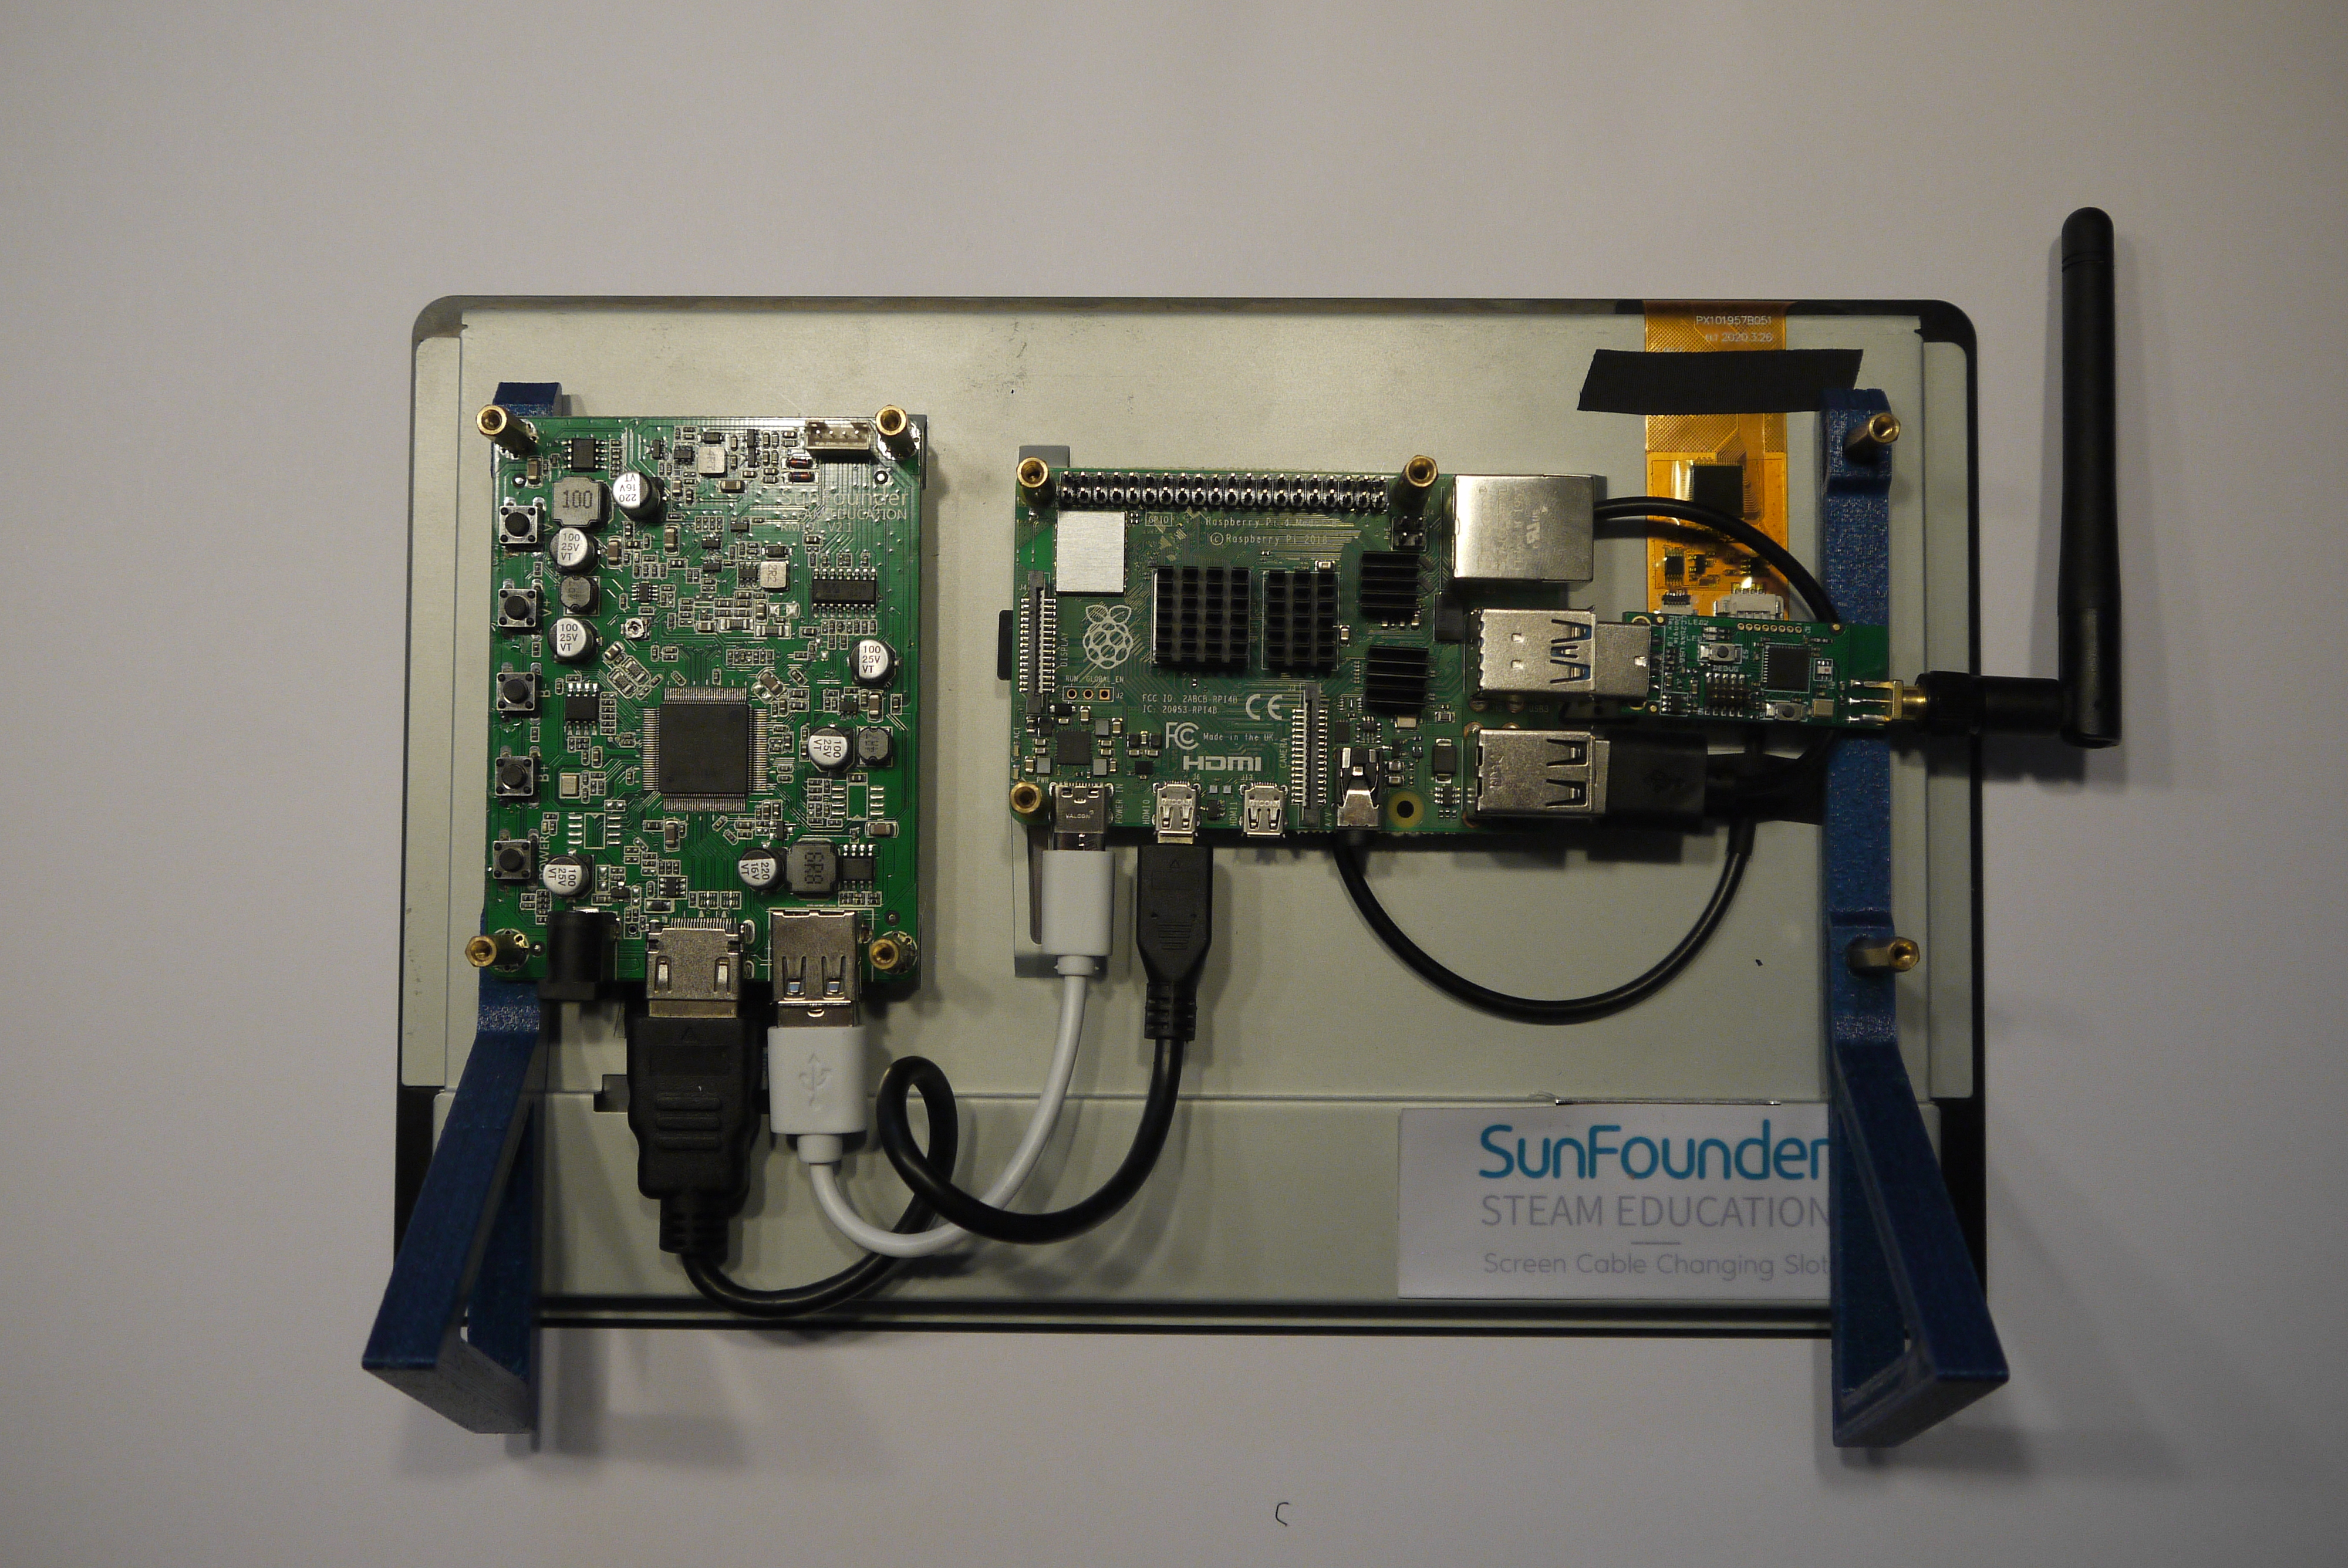
\includegraphics[width=1\textwidth]{img/prototype_back_detail.png}
		\caption[Detailansicht der Rückseite]{Detailansicht der Rückseite}
	\end{subfigure}
	\caption[Prototyp der Smart Home Zentrale]{Prototyp der Smart Home Zentrale}
	\label{prototype}
\end{figure}
\newpage
% Gehäuse
\subsection{Gehäuse}\label{hw_case}
% Erster Test
\subsubsection{Erster Test zur Fertigung des Gehäuses}\label{hw_case_ersterTest}
Zur Erstellung des Gehäuses haben wir die Maße des Bildschirms als Anhaltspunkt genommen. 
Die erste Messung haben wir mit einem Meterstab durchgeführt.
Der Bildschirm hatte an der Hinterseite eine Erhebung, weshalb wir diese ebenfalls ausgemessen haben. 
Die Maße beliefen sich nach der ersten Messung auf:
\begin{itemize}
	\item 255,5 mm Breite
	\item 167 mm Höhe
	\item Kantenradius 10 mm
\end{itemize}
\begin{figure}[H]
	\includegraphics[width=1\textwidth]{img/abmessungen_gehäuse.jpg}
	\caption[Abmessungen Bildschirm Rückseite]{Abmessungen Bildschirm Rückseite}
	\label{fig:screen-back-01}
\end{figure}
\noindent Anhand dieser Maße haben wir dann in Fusion 360 eine Grundplanzeichnung und ein 3D-Modell erstellt.\par	
\noindent Nach Überprüfung der Maße haben wir dann allerdings festgestellt, dass der zur Verfügung stehende 3D-Drucker, der Ender 3 Pro der Firma Creality3D, ein maximales Druckvolumen von 235 x 235 x 220 mm besitzt und somit das Gehäuse nicht wie ursprünglich geplant aus einem Stück, sondern in mehreren Teilen gedruckt werden muss. \\
\noindent Die ursprüngliche Konstruktion musste geändert werden. 
Das Gehäuse besteht nun aus vier Teilen, zwei davon bilden jeweils die Seitenwände, während zwei weitere den Deckel des Gehäuses bilden. 
Die Teile werden mit langen M3 Senkkopfschrauben verbunden, die zusätzlich als Verschluss des Gehäuses dienen.\par
\begin{figure}[H]
	\includegraphics[width=1\textwidth]{img/druck_gehäuse_001.png}
	\caption[Platzierung der beiden Gehäusewände in CURA]{Platzierung der beiden Gehäusewände in CURA}
	\label{fig:print-case-test_01}
\end{figure}
\begin{figure}[H]
	\includegraphics[width=1\textwidth]{img/druck_gehäuse_002.png}
	\caption[Verschiebung der Modelle entlang der Z-Achse um 45mm]{Verschiebung der Modelle entlang der Z-Achse um 45 mm}
	\label{fig:print-case-test_02}
\end{figure}
\begin{figure}[H]
	\includegraphics[width=1\textwidth]{img/druck_gehäuse_002.png}
	\caption[Slicen der Modelle]{Slicen der Modelle}
	\label{fig:print-case-test_03}
\end{figure}
\begin{figure}[H]
	\includegraphics[width=1\textwidth]{img/testdruck_an_bildschirm.jpg}
	\caption[Anlegen des Testdrucks]{Anlegen des Testdrucks}
	\label{fig:print-case-test_04}
\end{figure}
\noindent Um die Genauigkeit der Konstruktion zu testen, haben wir eine 5 Millimeter hohe Schablone ausgedruckt, die am Bildschirm ausprobiert wurde. 
Der Ausdruck entstand mit Hilfe des Slicers CURA (vgl. Abb. \ref{fig:print-case-test_01}: \nameref{fig:print-case-test_01}), in dem die Modelle der beiden Seitenteile so angeordnet wurden, dass lediglich 5 Millimeter des Teils im druckbaren Bereich des Druckers verblieben (vgl. Abb. \ref{fig:print-case-test_02}: \nameref{fig:print-case-test_02}). 
Anschließend haben wir die Teile noch auf dem Druckbett zentriert (vgl. Abb. \ref{fig:print-case-test_03}: \nameref{fig:print-case-test_03}).\\
\noindent Nach dem Ausdrucken war klar, dass die Maße des ersten Versuchs nicht genau genug waren (vgl. Abb. \ref{fig:print-case-test_04}: \nameref{fig:print-case-test_04}, weshalb wir zum Ausmessen einen digitaler Messschieber mit einer Nachkommastelle und einer  Genauigkeit von $\pm$ 0.2 mm verwendeten.
% Modellentwicklung am Objekt
\subsubsection{Modellentwicklung am Objekt}
Nachdem das Testmodell (vgl. Abbildung \ref{fig:print-case-test_04}) nicht zu 100 \% gepasst hat, hat Manuel Starz die Abmessungen neu geklärt und diese in Fusion 360 übertragen (vgl. \ref{case_footprint}). Um Material für den 3D-Druck zu sparen, wurde die Zeichnung dann im Maßstab 1:1 auf Papier gedruckt, ausgeschnitten und angelegt.\par
Da hier einige Maße noch nicht gestimmt haben, hat Manuel Starz den Plan überarbeitet (vgl. \ref{case_footprint_final}). Diese neuen Bemaßungen waren dann korrekt.\par
Daraufhin wurde dann die Zeichnung in zwei eigenständige Dateien gesplittet, um die linke und die rechte Seite des Gehäuses zu konstruieren.\par
Die Grundabmessung des Bildschirms werden in Fusion 360 als neue Zeichnung angelegt. Hierzu wurde ein einfaches Rechteck mit den entsprechenden Außenmaßen angelegt (vlg. \ref{fig:design-case-01}). Anschließend wurden die Ecken mit einem Radius von 7mm abgerundet. (vgl. \ref{fig:design-case-02}). Abschließend wurde die Zeichnung in der Mitte geteilt, um die beiden Hälften des Gehäuses unabhängig\par
\begin{figure}[h!tb]
	\begin{subfigure}[b]{.5\linewidth}
		\includegraphics[width=1\textwidth]{img/konstruktion_gehaeuse_001.png}
		\caption[Zeichnen der Außenmaße]{Zeichnen der Außenmaße}
		\label{fig:design-case-01}
	\end{subfigure}
	\begin{subfigure}[b]{.5\linewidth}
		\includegraphics[width=1\textwidth]{img/konstruktion_gehaeuse_002.png}
		\caption[Abrunden der Ecken]{Abrunden der Ecken}
		\label{fig:design-case-02}
	\end{subfigure}
	\begin{subfigure}[b]{.5\linewidth}
		\includegraphics[width=1\textwidth]{img/konstruktion_gehaeuse_003.png}
		\caption[Zeichnen der Auflageflächen für das Gehäuse]{Zeichnen der Auflageflächen}
		\label{fig:design-case-03}
	\end{subfigure}
	\caption[Grundzeichnung als Basis des Modells]{Grundzeichnung als Basis des Modells}
	\label{fig:design-case-base}
\end{figure}\par
Die so entstandene Zeichnung (vgl. \ref{fig:design-case-03}) wurde dann in eine weitere Datei kopiert um als Grundlage für die beiden geteilten Seitenteile zu dienen. Von hier aus wurden die beiden Wand-Teile mehr oder weniger unabhängig voneinander entworfen.\par
\paragraph{Linkes Wandteil}
Beim linken Wandteil wurde der entsprechende Teil der Zeichnung um 2 mm entlang der Z-Achse extrudiert (vgl. \ref{fig:design-left-01}). Auf der erhöhten Seite wurde darauf hin eine weitere Zeichnung gelegt, die die Bleche an der Rückseite des Bildschirms überdecken sollte (vgl. \ref{fig:design-left-02}), die dann wie zuvor um 3 mm entlang der Z-Achse extrudiert wurde (vgl. \ref{fig:design-left-03}). Diese sollte dem Gehäuse genug Auflagefläche an dem Bildschirm bieten, um die Verklebung so stark wie möglich zu machen. Auf die nun entstandene erhöhte Seite wurde eine Zeichnung der ,,tatsächlichen'' Wandstärke von 3 mm erstellt (vgl. \ref{fig:design-left-04}). Diese wurde dann um 6 mm entlang der Z-Achse extrudiert, um für die Verbinder genügend Platz vor dem klobigen Blechbereich im unteren Teil des Bildschirms zu bieten (vgl. \ref{fig:design-left-05}). Auf die nun obenliegende Seite wurde die Zeichnung der Verbindungsstücke gelegt (vgl. \ref{fig:design-left-06}) und um 19 mm entlang der Z-Achse extrudiert (vgl. \ref{fig:design-left-07}) und im Kreismittelpunkt der Zeichnungen eine Bohrung für M3-Gewinde gesetzt (vgl. \ref{fig:design-left-08}). Auf die nun  entstandene Oberfläche wurde die Zeichnung für die Deckelverbindung gesetzt (vgl. \ref{fig:design-left-09}), um 25 mm entlang der Z-Achse extrudiert (vgl. \ref{fig:design-left-10}) und ebenfalls mit Bohrungen für M3-Gewinde versehen (vgl. \ref{fig:design-left-11}).
%beschreibungstext links
\begin{figure}[h!tb]
	\begin{subfigure}[t]{.3\linewidth}
		\includegraphics[width=\linewidth]{img/konstruktion_gehaeuse_links_001.png}
		\caption[Extrusion der Grundzeichnung]{Extrusion der Grundzeichnung}
		\label{fig:design-left-01}
	\end{subfigure}
	\begin{subfigure}[t]{.3\linewidth}
		\includegraphics[width=\linewidth]{img/konstruktion_gehaeuse_links_002.png}
		\caption[Erstellung der Folgezeichnung um Blech]{Erstellung der Folgezeichnung um Blech}
		\label{fig:design-left-02}
	\end{subfigure}
	\begin{subfigure}[t]{.3\linewidth}
		\includegraphics[width=\linewidth]{img/konstruktion_gehaeuse_links_003.png}
		\caption[Extrusion der neuen Zeichnung]{Extrusion der neuen Zeichnung}
		\label{fig:design-left-03}
	\end{subfigure}
	\begin{subfigure}[t]{.3\linewidth}
		\includegraphics[width=\linewidth]{img/konstruktion_gehaeuse_links_004.png}
		\caption[Zeichnung der Hauptwandstärke]{Zeichnung der Hauptwandstärke}
		\label{fig:design-left-04}
	\end{subfigure}
	\begin{subfigure}[t]{.3\linewidth}
		\includegraphics[width=\linewidth]{img/konstruktion_gehaeuse_links_005.png}
		\caption[Extrusion der Hauptwand]{Extrusion der Hauptwand}
		\label{fig:design-left-05}
	\end{subfigure}
	\begin{subfigure}[t]{.3\linewidth}
		\includegraphics[width=\linewidth]{img/konstruktion_gehaeuse_links_006.png}
		\caption[Zeichnung der Verbindungsstücke]{Zeichnung der Verbindungsstücke}
		\label{fig:design-left-06}
	\end{subfigure}
	\begin{subfigure}[t]{.3\linewidth}
		\includegraphics[width=\linewidth]{img/konstruktion_gehaeuse_links_007.png}
		\caption[Extrusion der Hauptwand mit Verbindungsstücken]{Extrusion der Hauptwand mit Verbindungsstücken}
		\label{fig:design-left-07}
	\end{subfigure}
	\begin{subfigure}[t]{.3\linewidth}
		\includegraphics[width=\linewidth]{img/konstruktion_gehaeuse_links_008.png}
		\caption[Bohrung für Schrauben]{Bohrung für Schrauben}
		\label{fig:design-left-08}
	\end{subfigure}
	\begin{subfigure}[t]{.3\linewidth}
		\includegraphics[width=\linewidth]{img/konstruktion_gehaeuse_links_009.png}
		\caption[Zeichnung der Deckelverbindung]{Zeichnung der Deckelverbindung}
		\label{fig:design-left-09}
	\end{subfigure}
	\begin{subfigure}[t]{.3\linewidth}
		\includegraphics[width=\linewidth]{img/konstruktion_gehaeuse_links_010.png}
		\caption[Extrusion der Hauptwand mit Deckelverbindung]{Extrusion der Hauptwand mit Deckelverbindung}
		\label{fig:design-left-10}
	\end{subfigure}
	\begin{subfigure}[t]{.3\linewidth}
		\includegraphics[width=\linewidth]{img/konstruktion_gehaeuse_links_011.png}
		\caption[Bohrungen der Deckelverbindung]{Bohrungen der Deckelverbindung}
		\label{fig:design-left-11}
	\end{subfigure}
	\caption[Entwurf des linken Wandteils]{Entwurf des linken Wandteils}
	\label{fig:design-left}
\end{figure}\par
\paragraph{Rechtes Wandteil}

\newpage
% Erstellung des Modells
\subsubsection{Herstellung des Gehäuses}\label{hw_case_herstellung}
Zur Herstellung des Gehäuses kommt ein 3D-Drucker der Marke Creality 3D zum Einsatz. 
Der stark modifizierte Ender 3 Pro von Manuel Starz (vgl. \ref{fig:ender3}) druckt die zuvor erstellten STL-Dateien mit PETG-Filament der Firma dasfilament. 
Der für den 3D-Druck nötige G-Code wird mit Ultimaker CURA generiert und mit Hilfe von OctoPrint (vgl. \ref{fig:octoprint}) an den Drucker übertragen. Das Gehäuse besteht aus vier Einzelteilen, je zwei Teile für die Seitenwände und zwei Teile für den Deckel.\par
\begin{figure}[h!tb]
	\begin{center}
	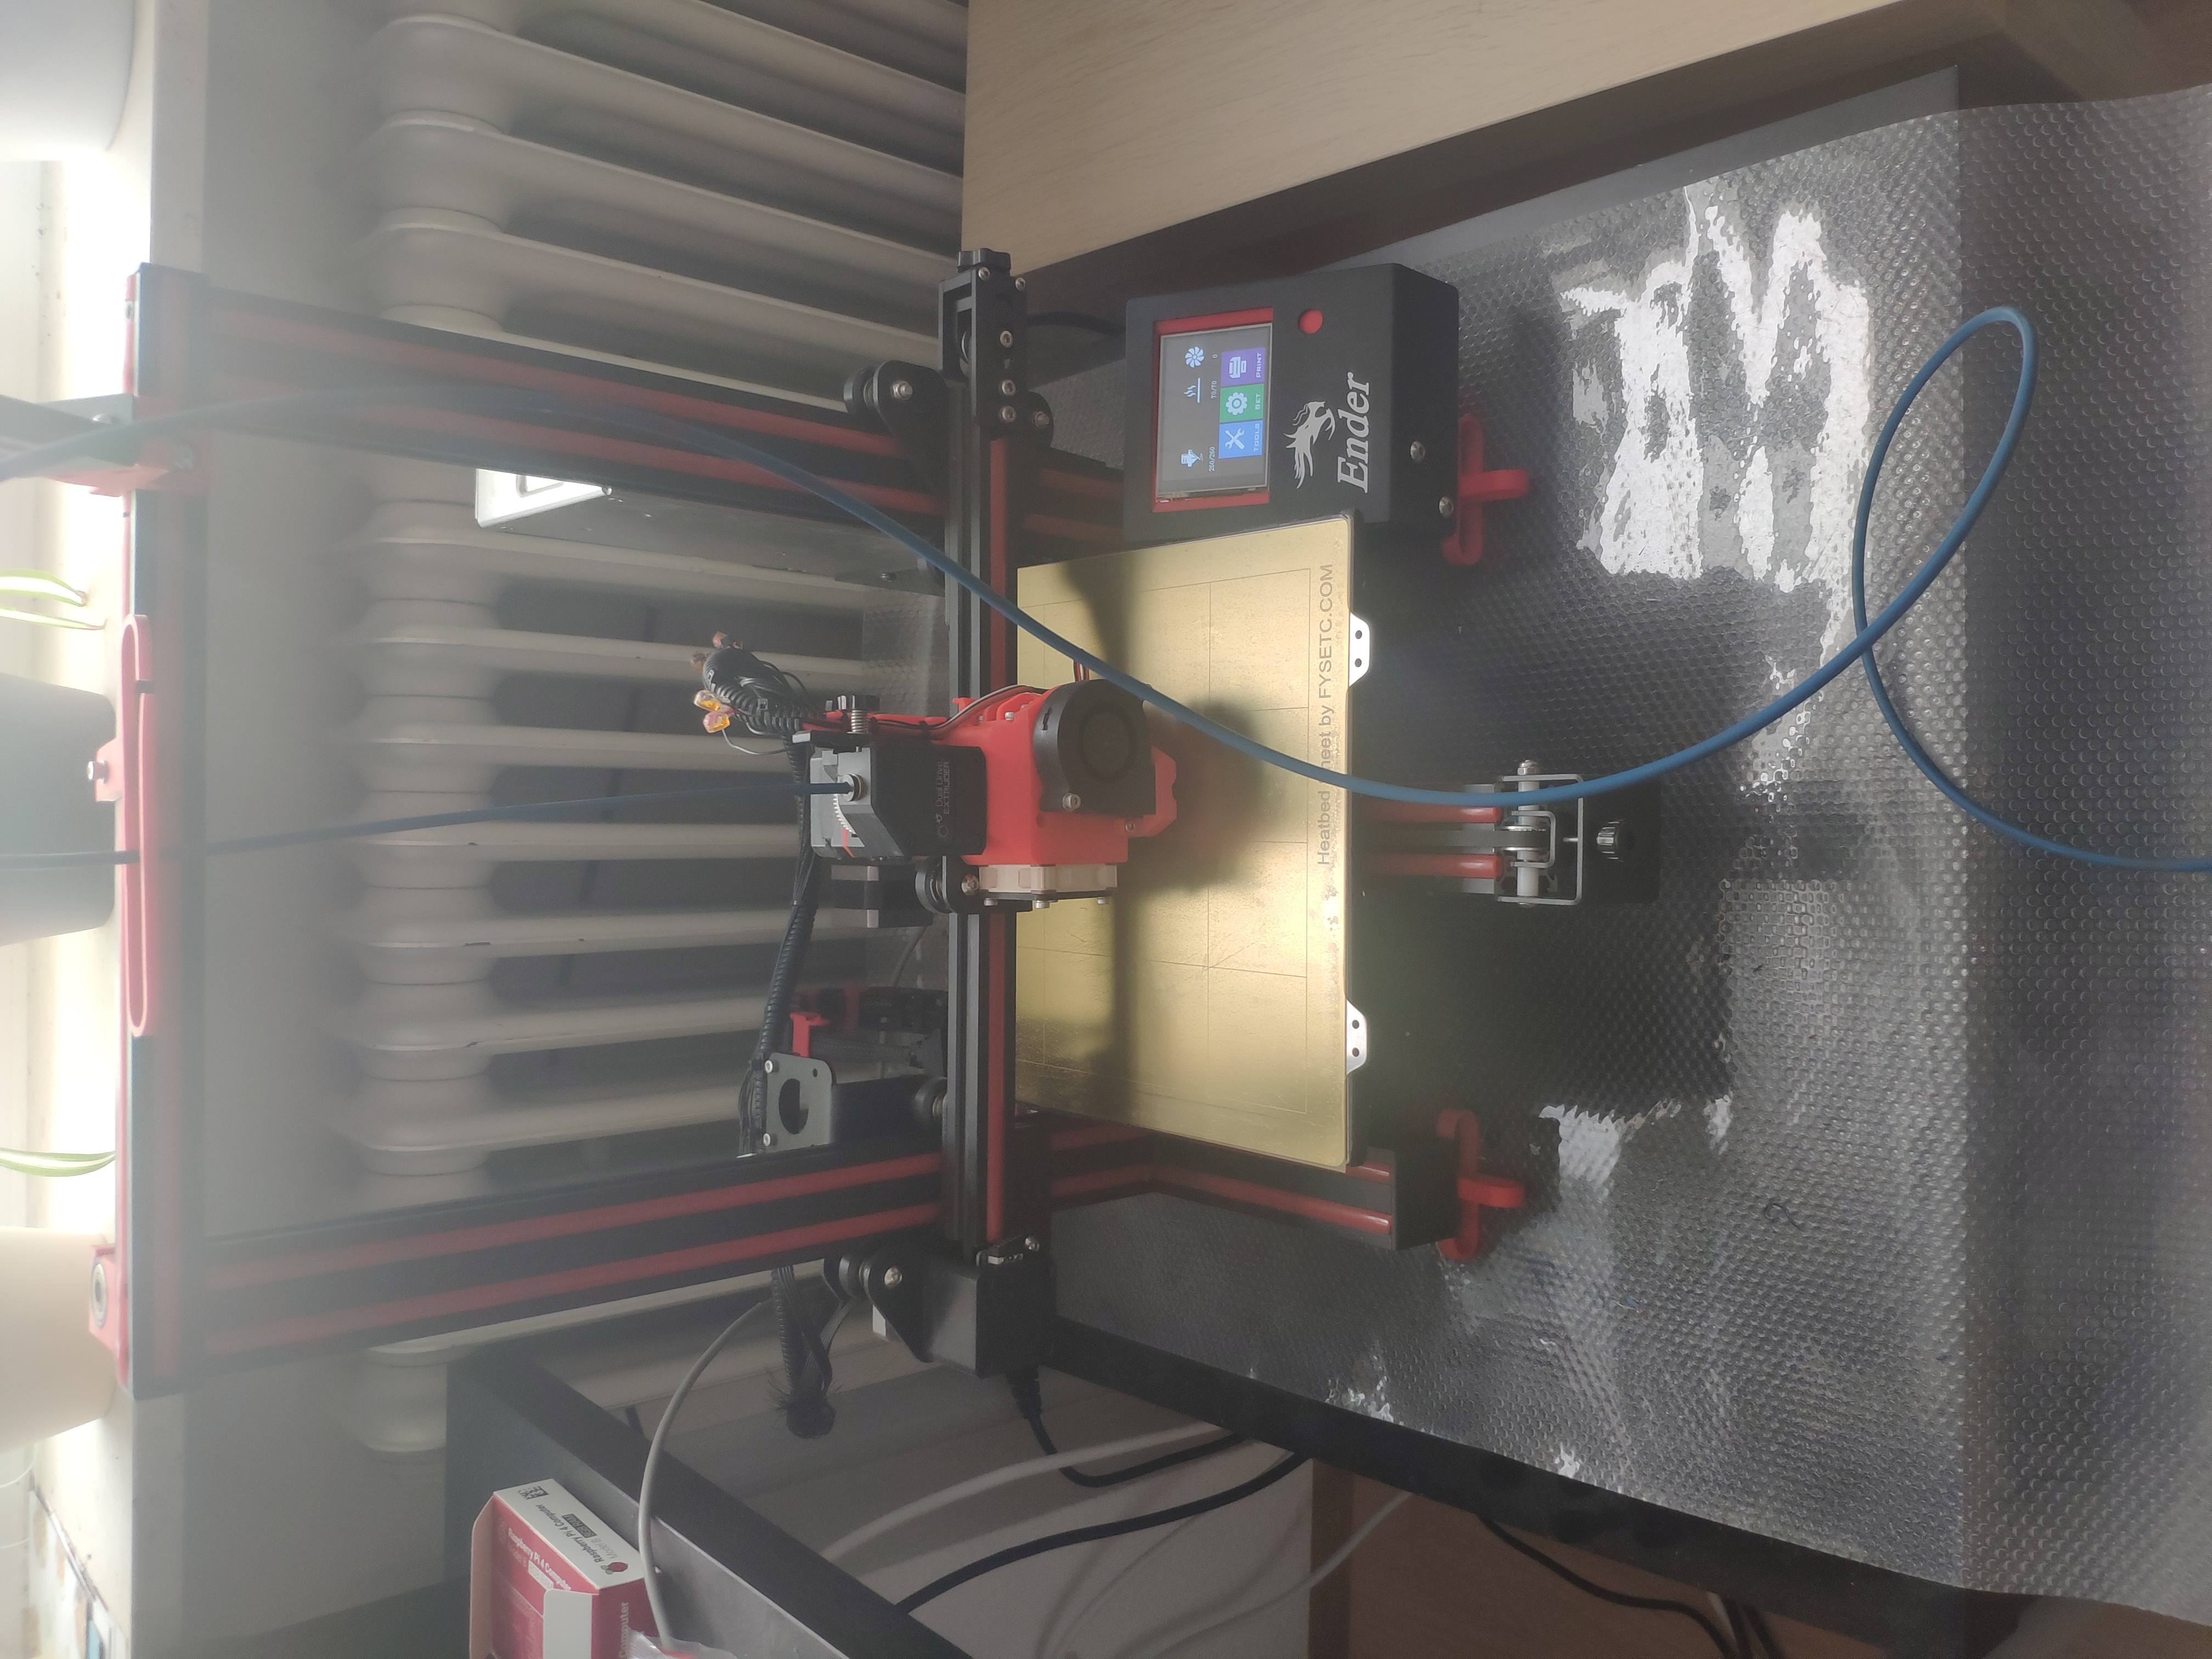
\includegraphics[width=.5\textwidth,angle=270]{img/ender3pro_mod.jpg}
	\end{center}
	\caption[3D-Drucker Ender 3 Pro (mod)]{3D-Drucker Ender 3 Pro (mod)}
	\label{fig:ender3}
\end{figure}
\begin{figure}[h!tb]
	\includegraphics[width=1\textwidth]{img/gehäusedruck_octoprint_01.png}
	\caption[OctoPrint-Weboberfläche]{OctoPrint-Weboberfläche}
	\label{fig:octoprint}
\end{figure}
\noindent Die gedruckten Teile (vgl. \ref{fig:printet_parts}) werden dann zum Teil mit Zwei-Komponenten-Epoxidkleber verbunden (vgl. \ref{fig:glued_parts}) und mit Hilfe von Schleifpapier und einigen Schichten Klarlack zu einem klavierlackähnlichen Finish veredelt (vgl. \ref{filed_and_painted_parts}). 
Die Seitenwände werden dann mit dem Bildschirm mit Hilfe des Zwei-Komponenten-Epoxidklebers und Heißkleber permanent verklebt (vgl. \ref{fig:finished_case_front}).
Danach wurden die Platinen und Kabel im Gehäuse angebracht (vgl. \ref{fig:finished_case_front}). 
Die Rückseite besteht der Einfachheit halber aus zwei identischen, punktsymmetrischen Teilen, die ebenfalls miteinander verklebt wurden.\par
\begin{figure}[h!tb]
	\begin{subfigure}[b]{0.5\linewidth}
		\centering
		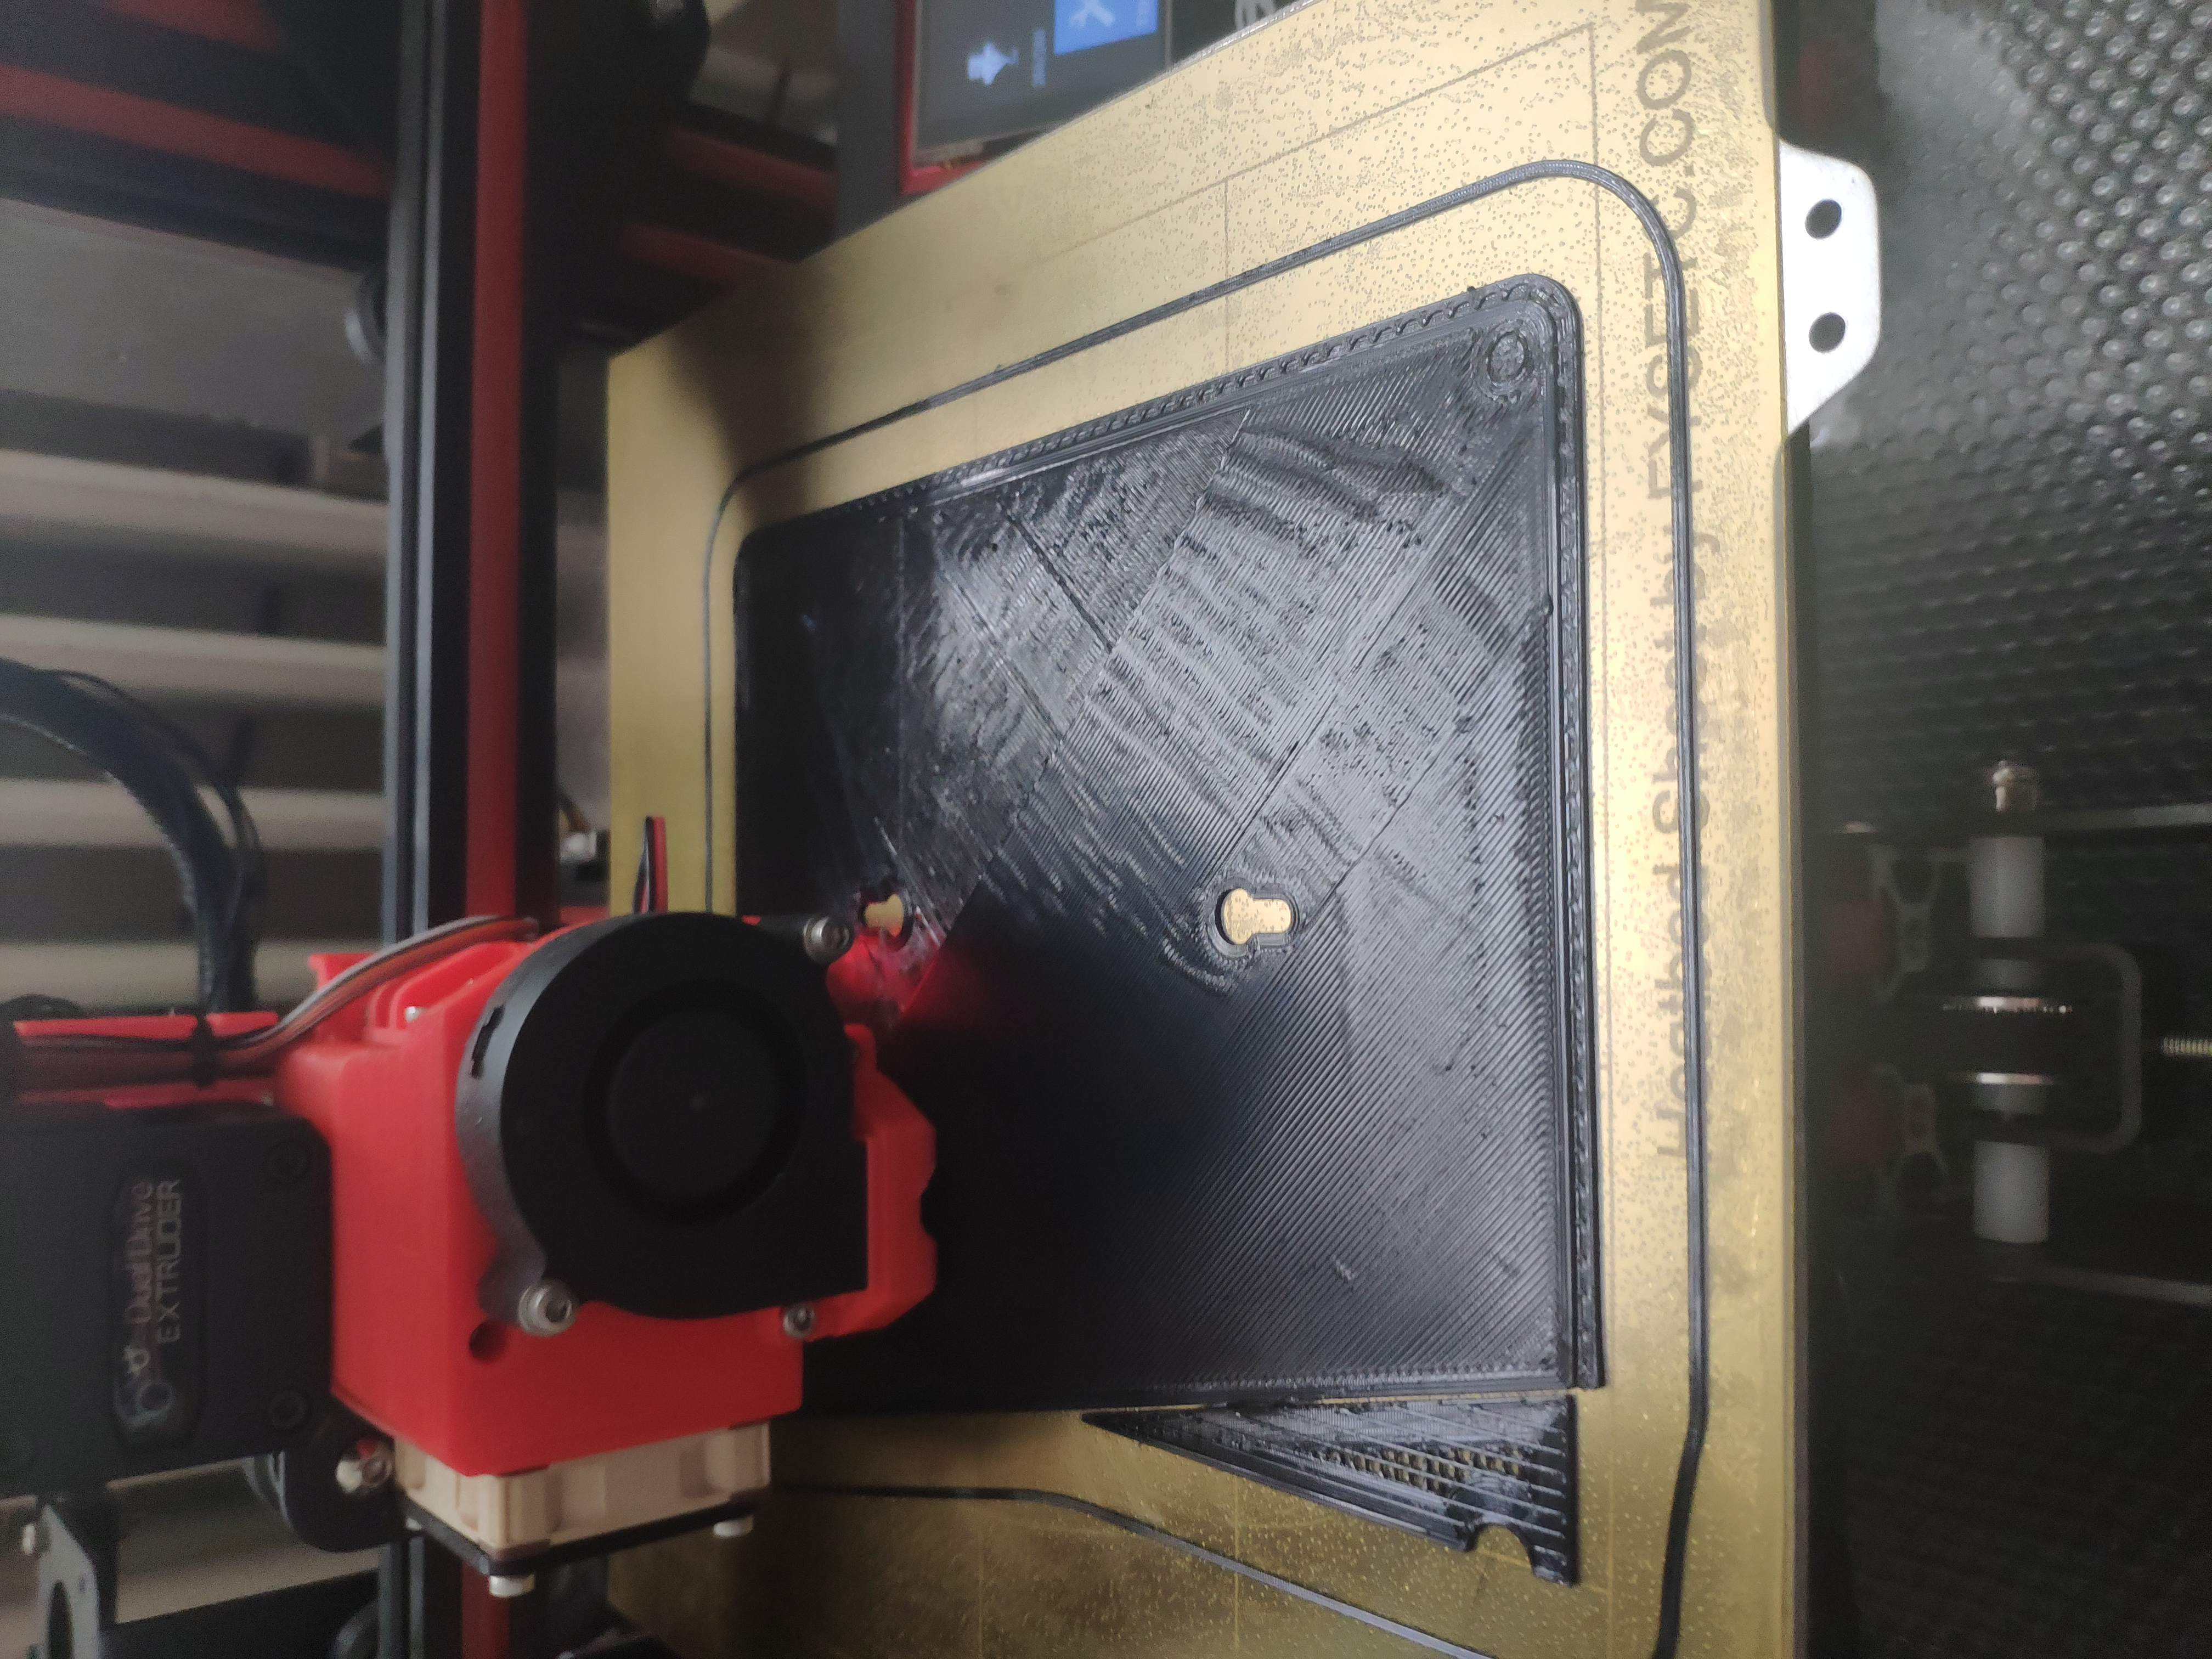
\includegraphics[width=1\textwidth,angle=270]{img/druck_deckel.jpg}
		\caption[Druck eines der Deckel-Teile]{Druck eines der Deckel-Teile}
	\end{subfigure}
	\begin{subfigure}[b]{0.5\linewidth}
		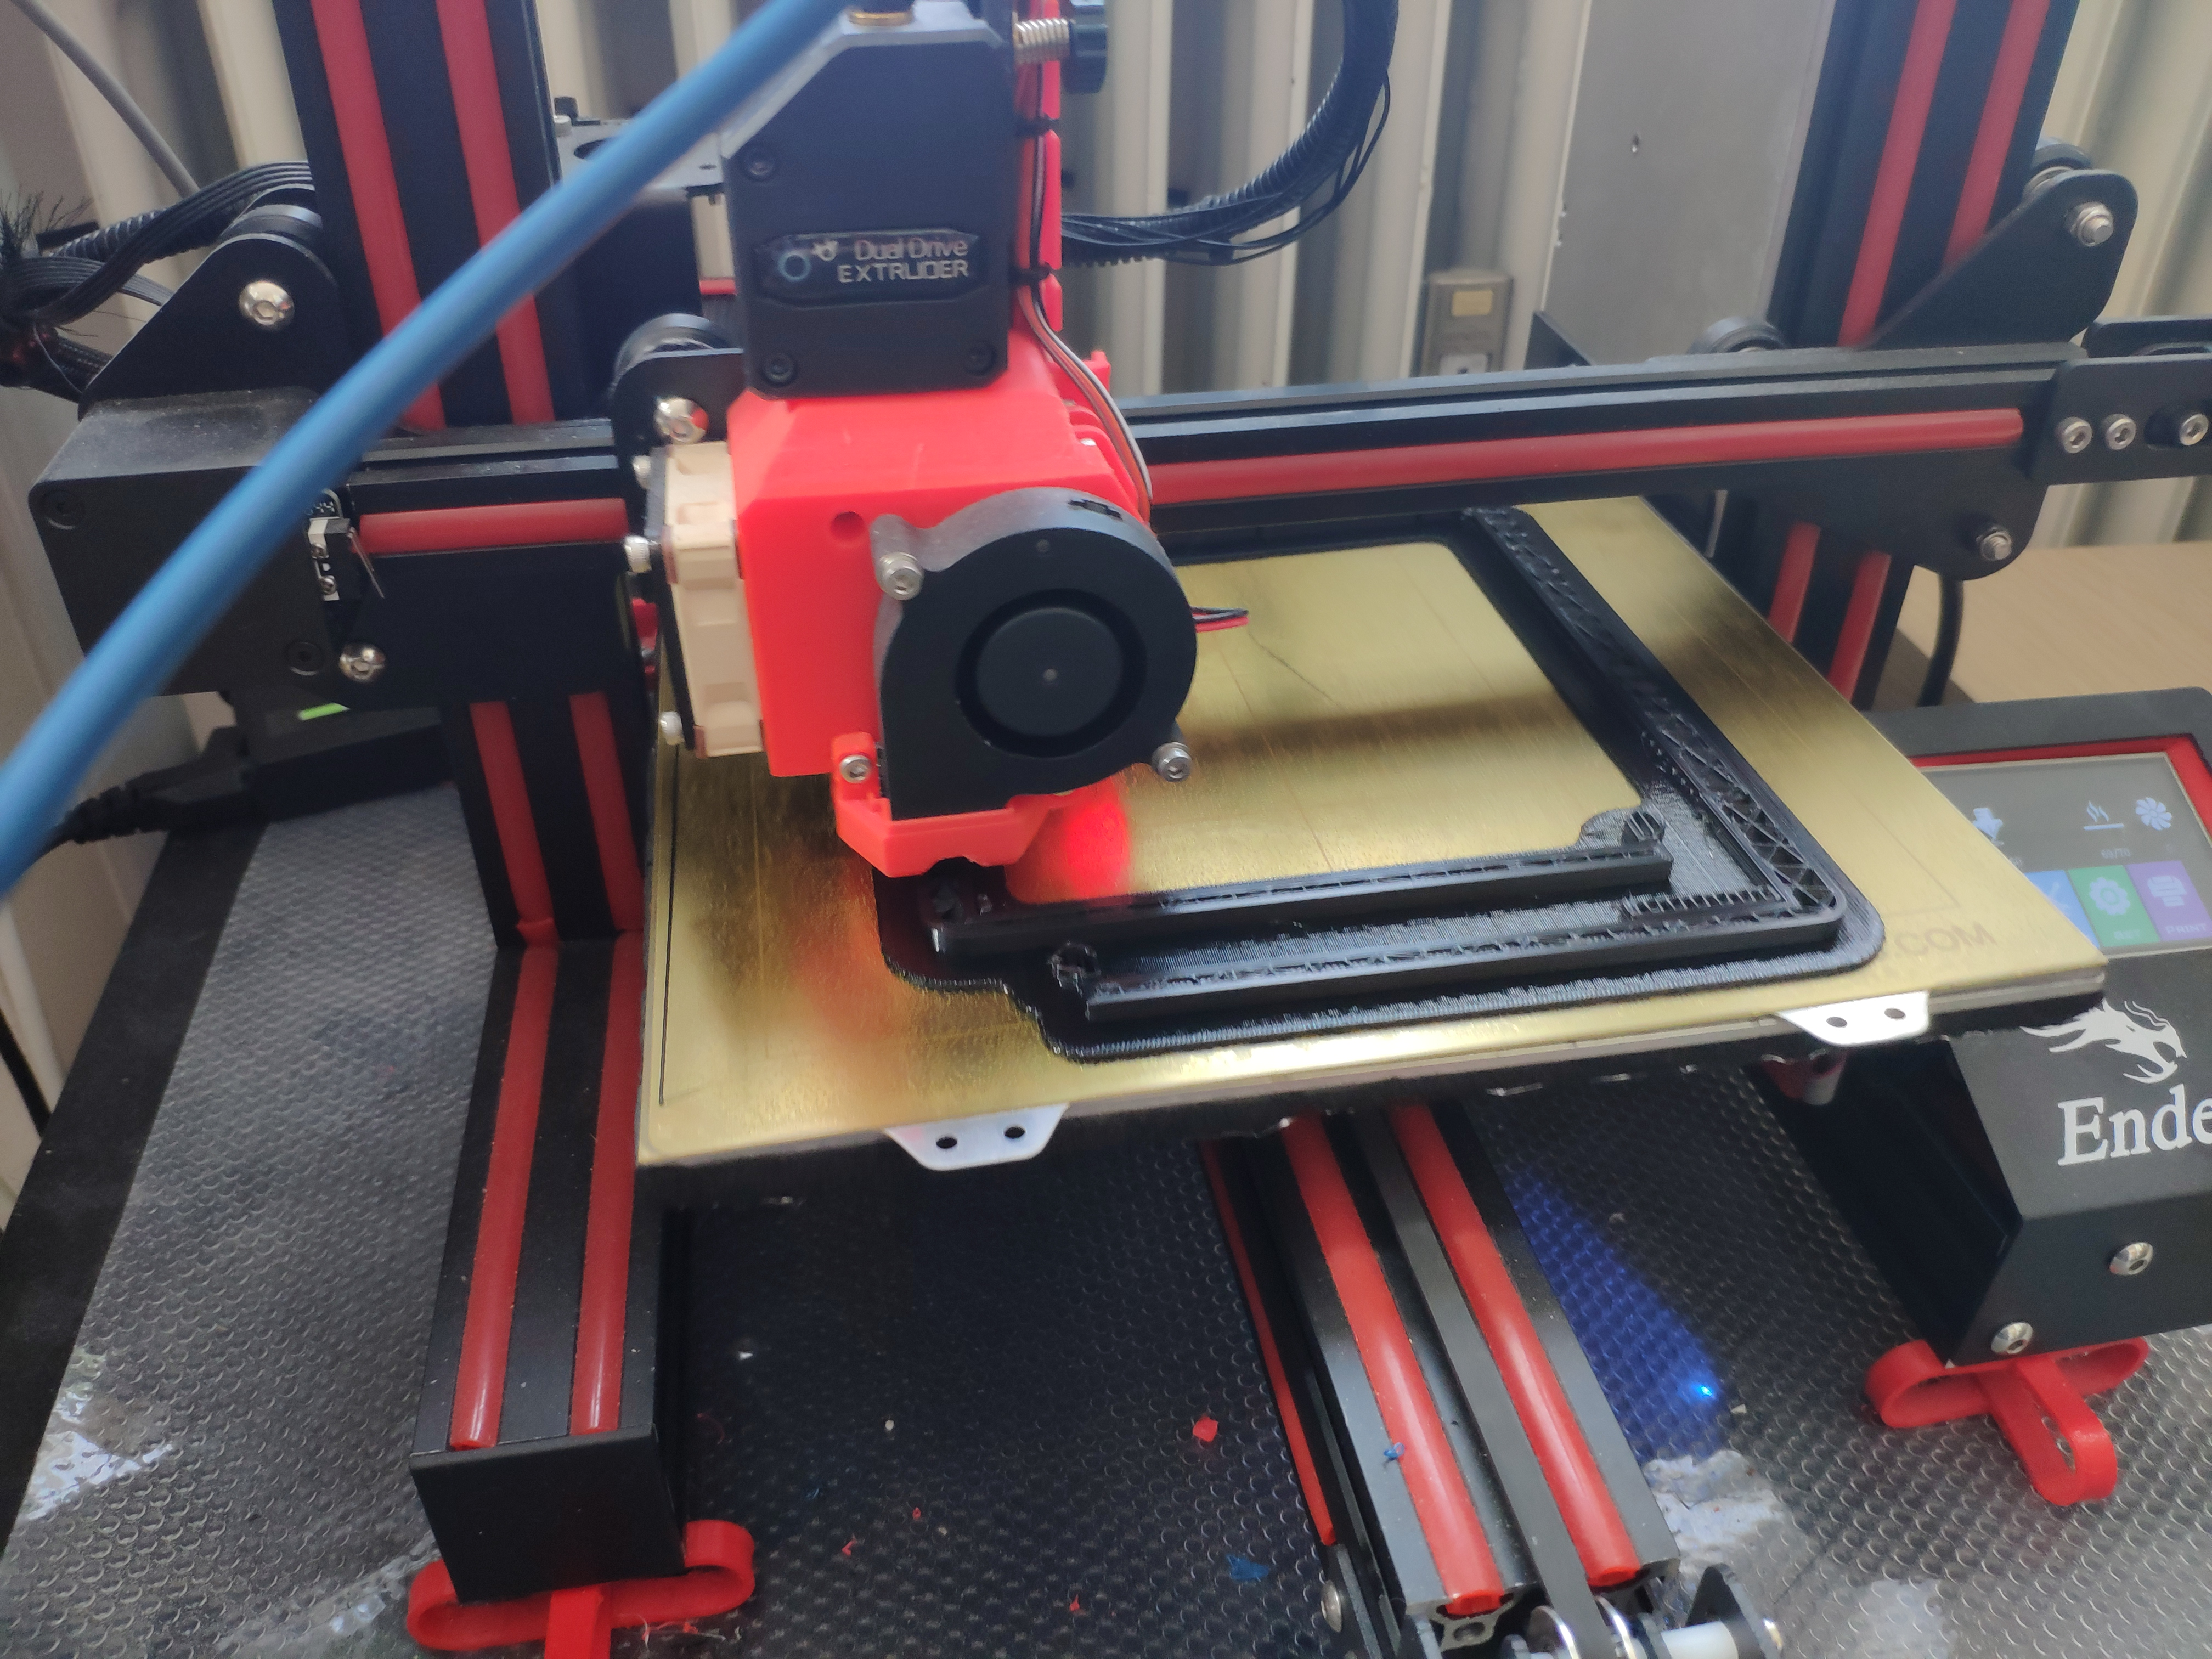
\includegraphics[width=1\textwidth]{img/druck_waende.jpg}
		\caption[Druck der Wand-Teile]{Druck der Wand-Teile}
	\end{subfigure}
	\caption[Das Gehäuse entsteht]{Das Gehäuse entsteht}
	\label{fig:printing_parts}
\end{figure}
\par
\begin{figure}[h!tb]
	\centering
	\begin{subfigure}[b]{0.3\linewidth}
		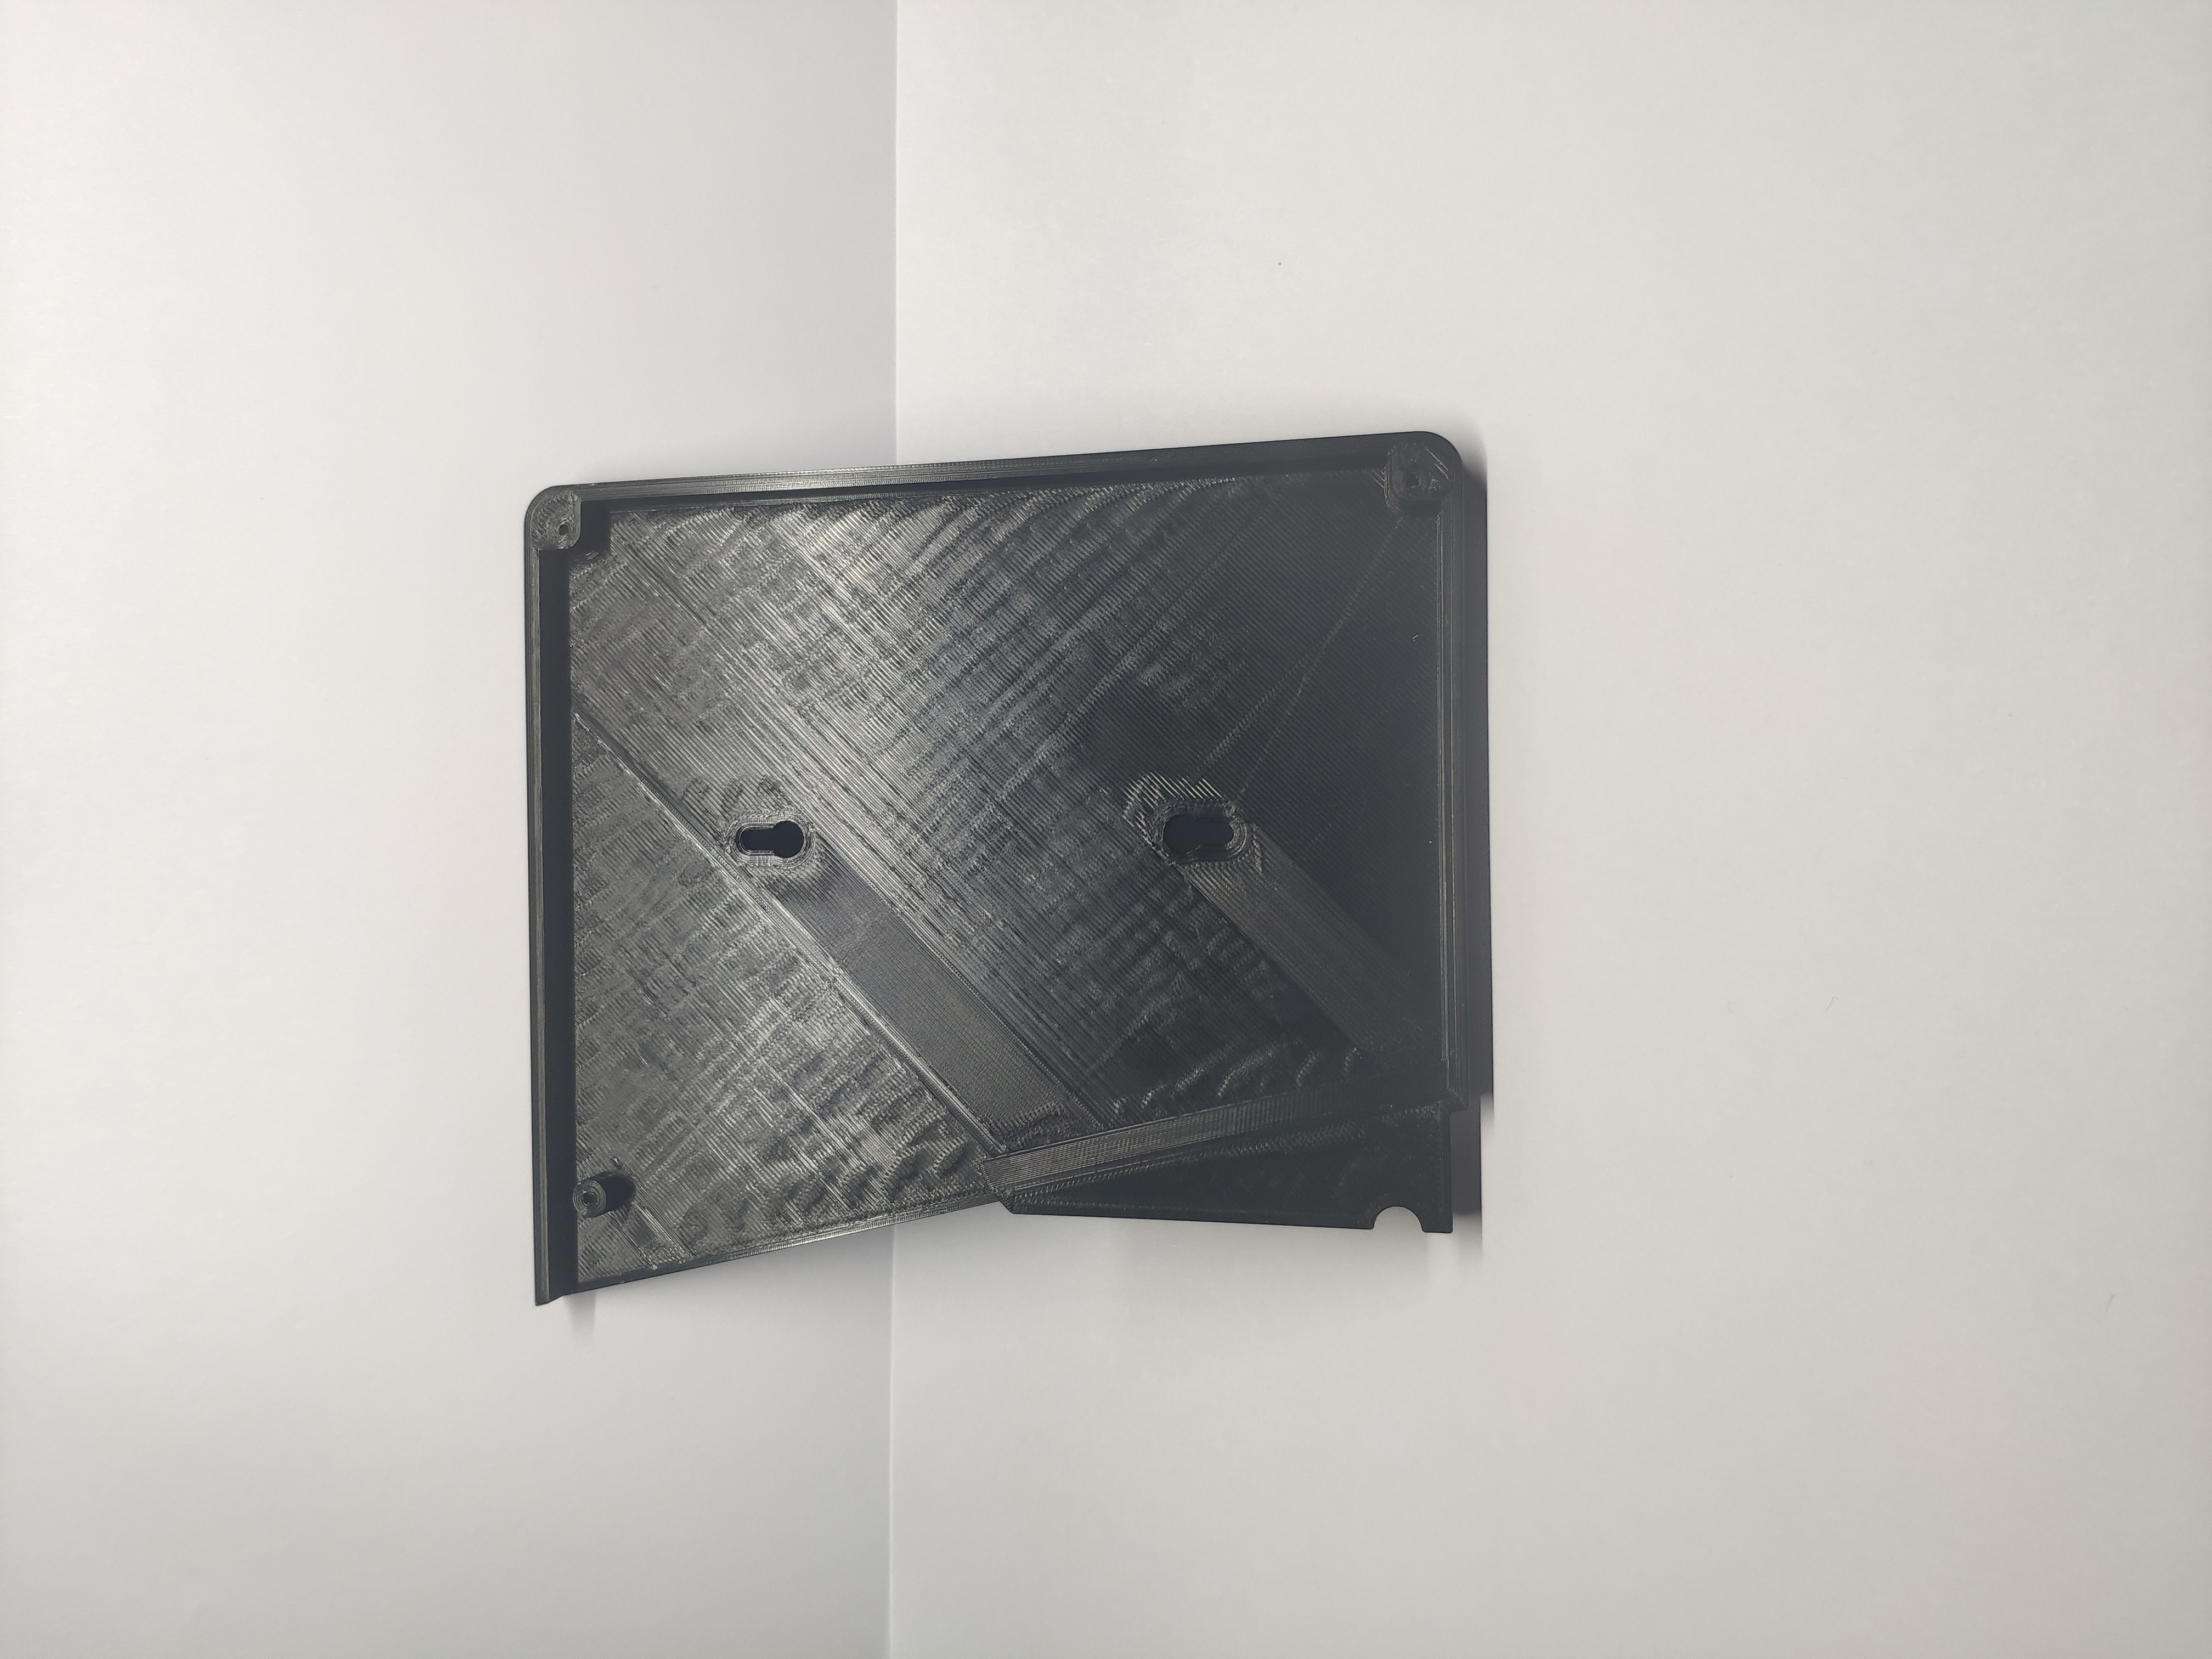
\includegraphics[width=1\linewidth,angle=270]{img/gehauese_rueck.jpg}
		\caption[Rückseite]{Rückseite}
		\label{printet_parts_back}
	\end{subfigure}
	\begin{subfigure}[b]{0.3\linewidth}
		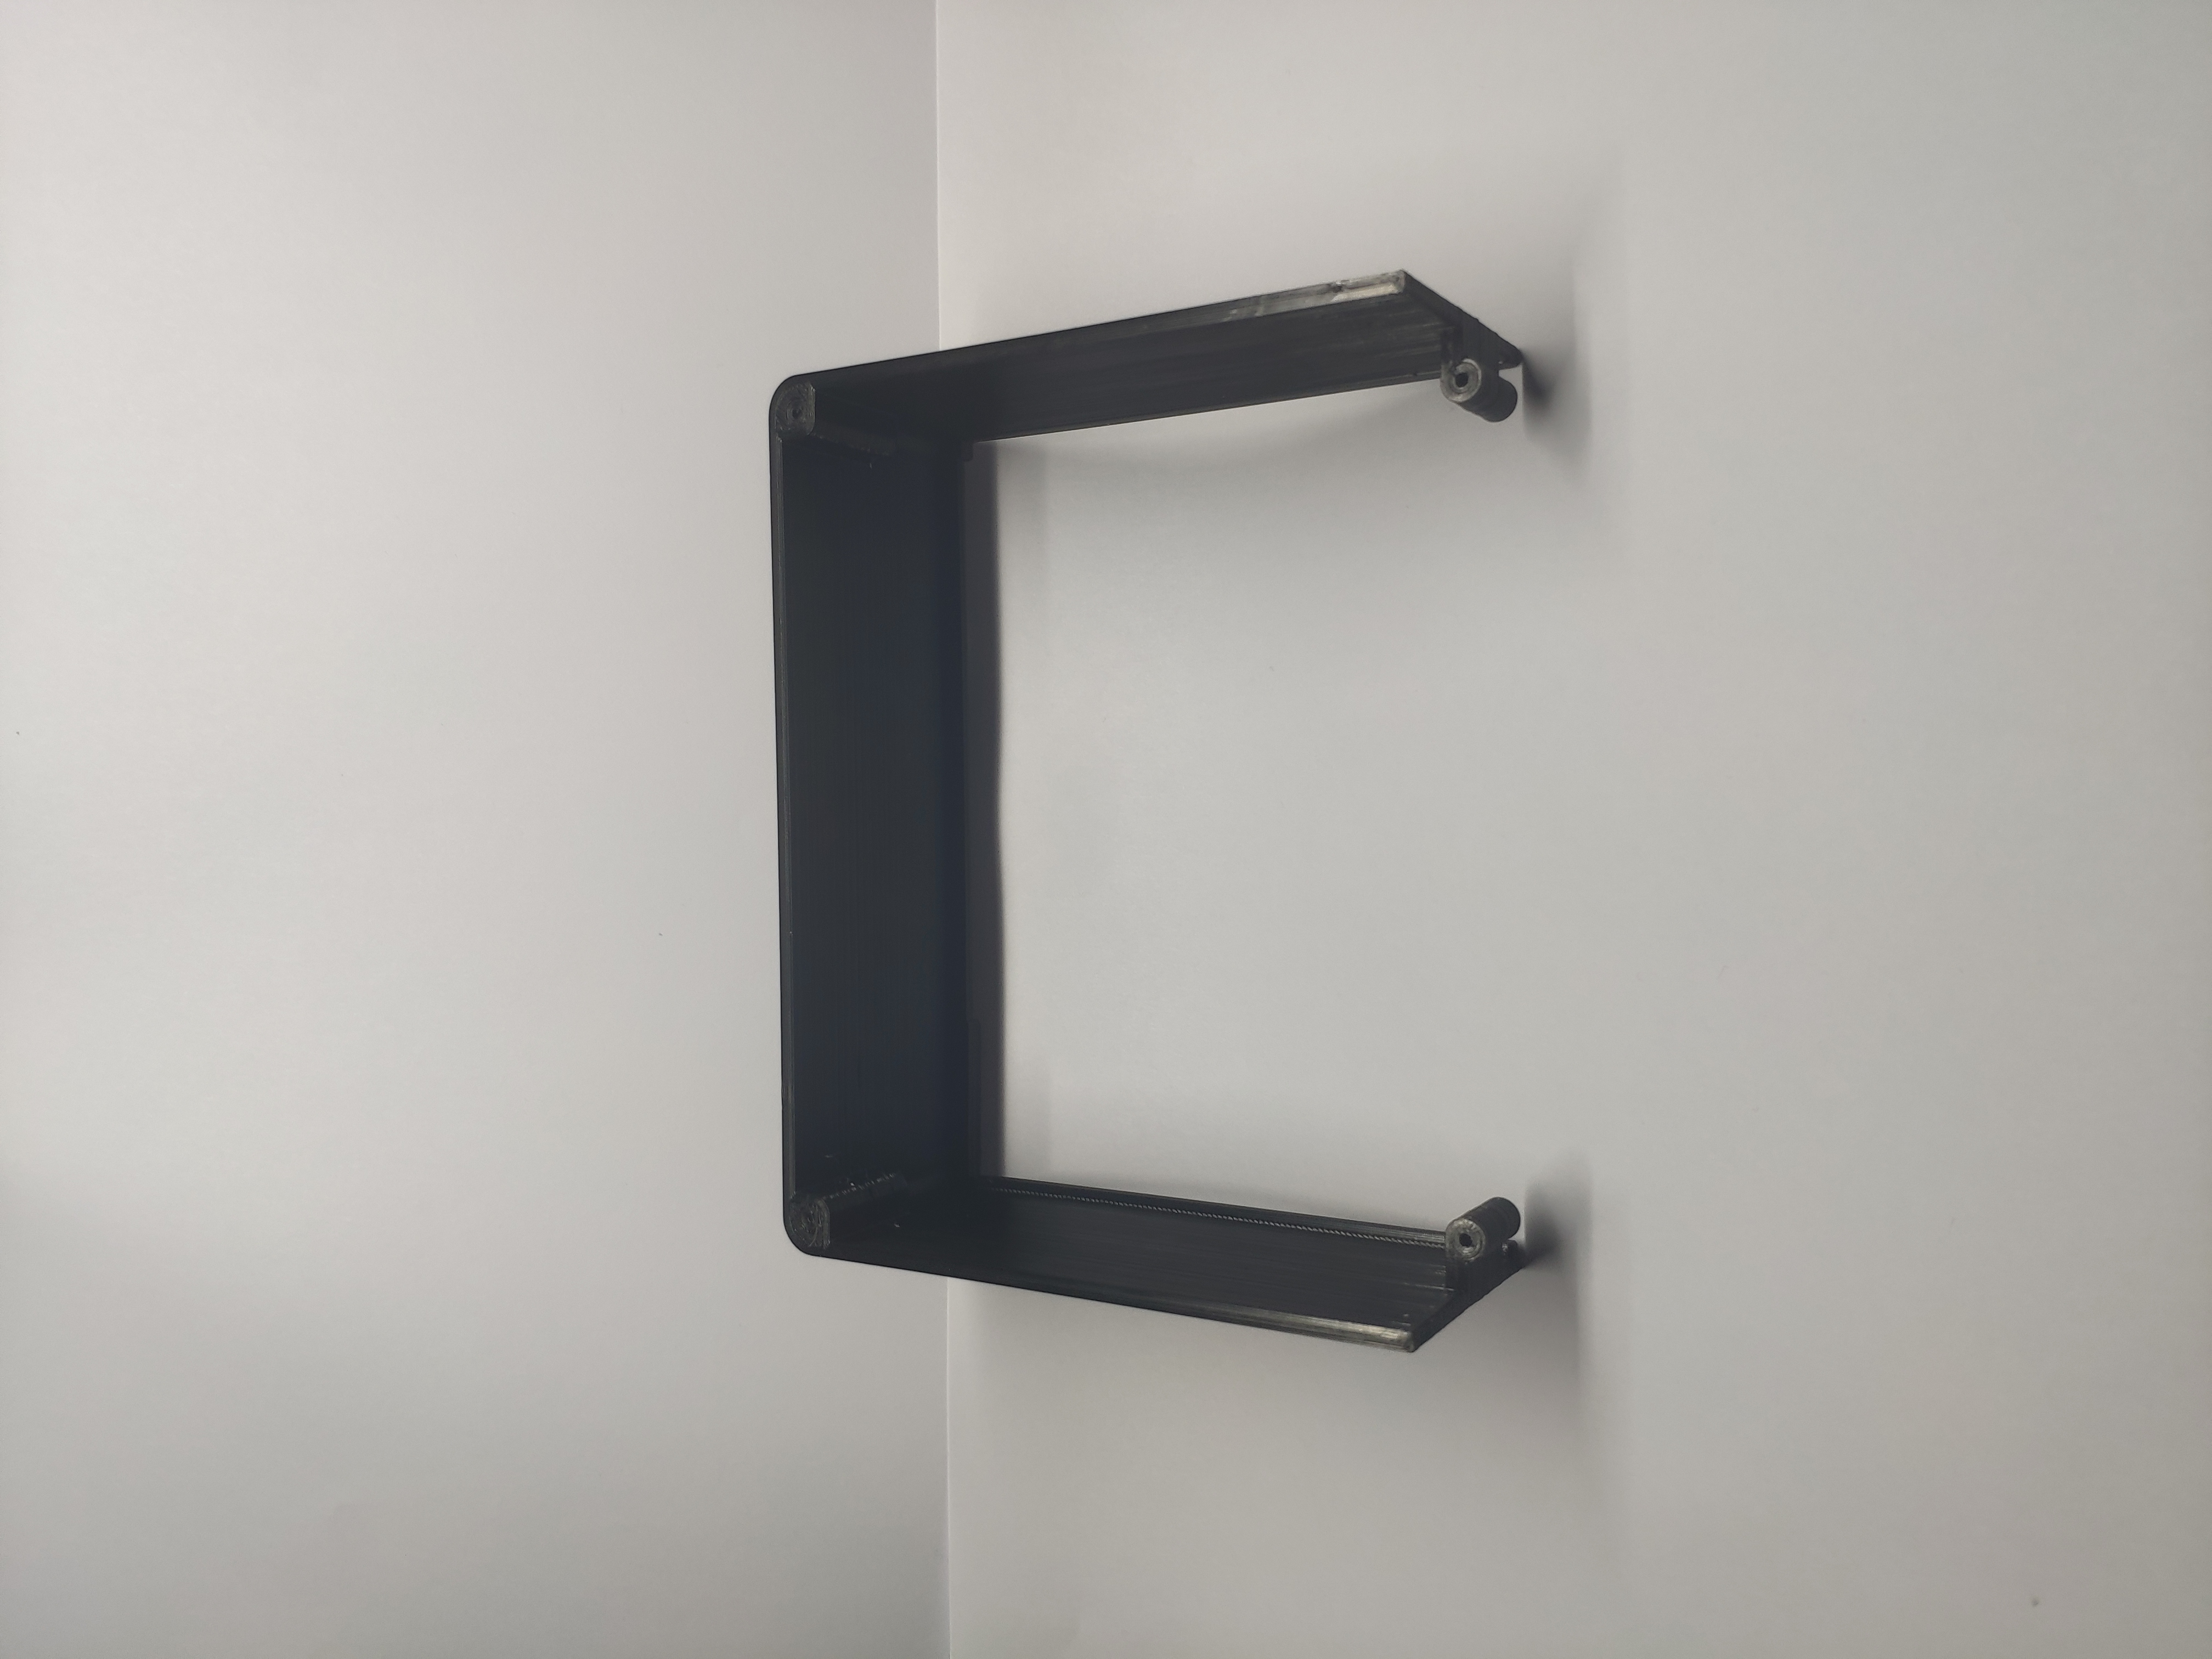
\includegraphics[width=1\linewidth,angle=270]{img/gehauese_links.jpg}
		\caption[Linke Seite]{Linke Seite}
		\label{printet_parts_left}
	\end{subfigure}
	\begin{subfigure}[b]{0.3\linewidth}
		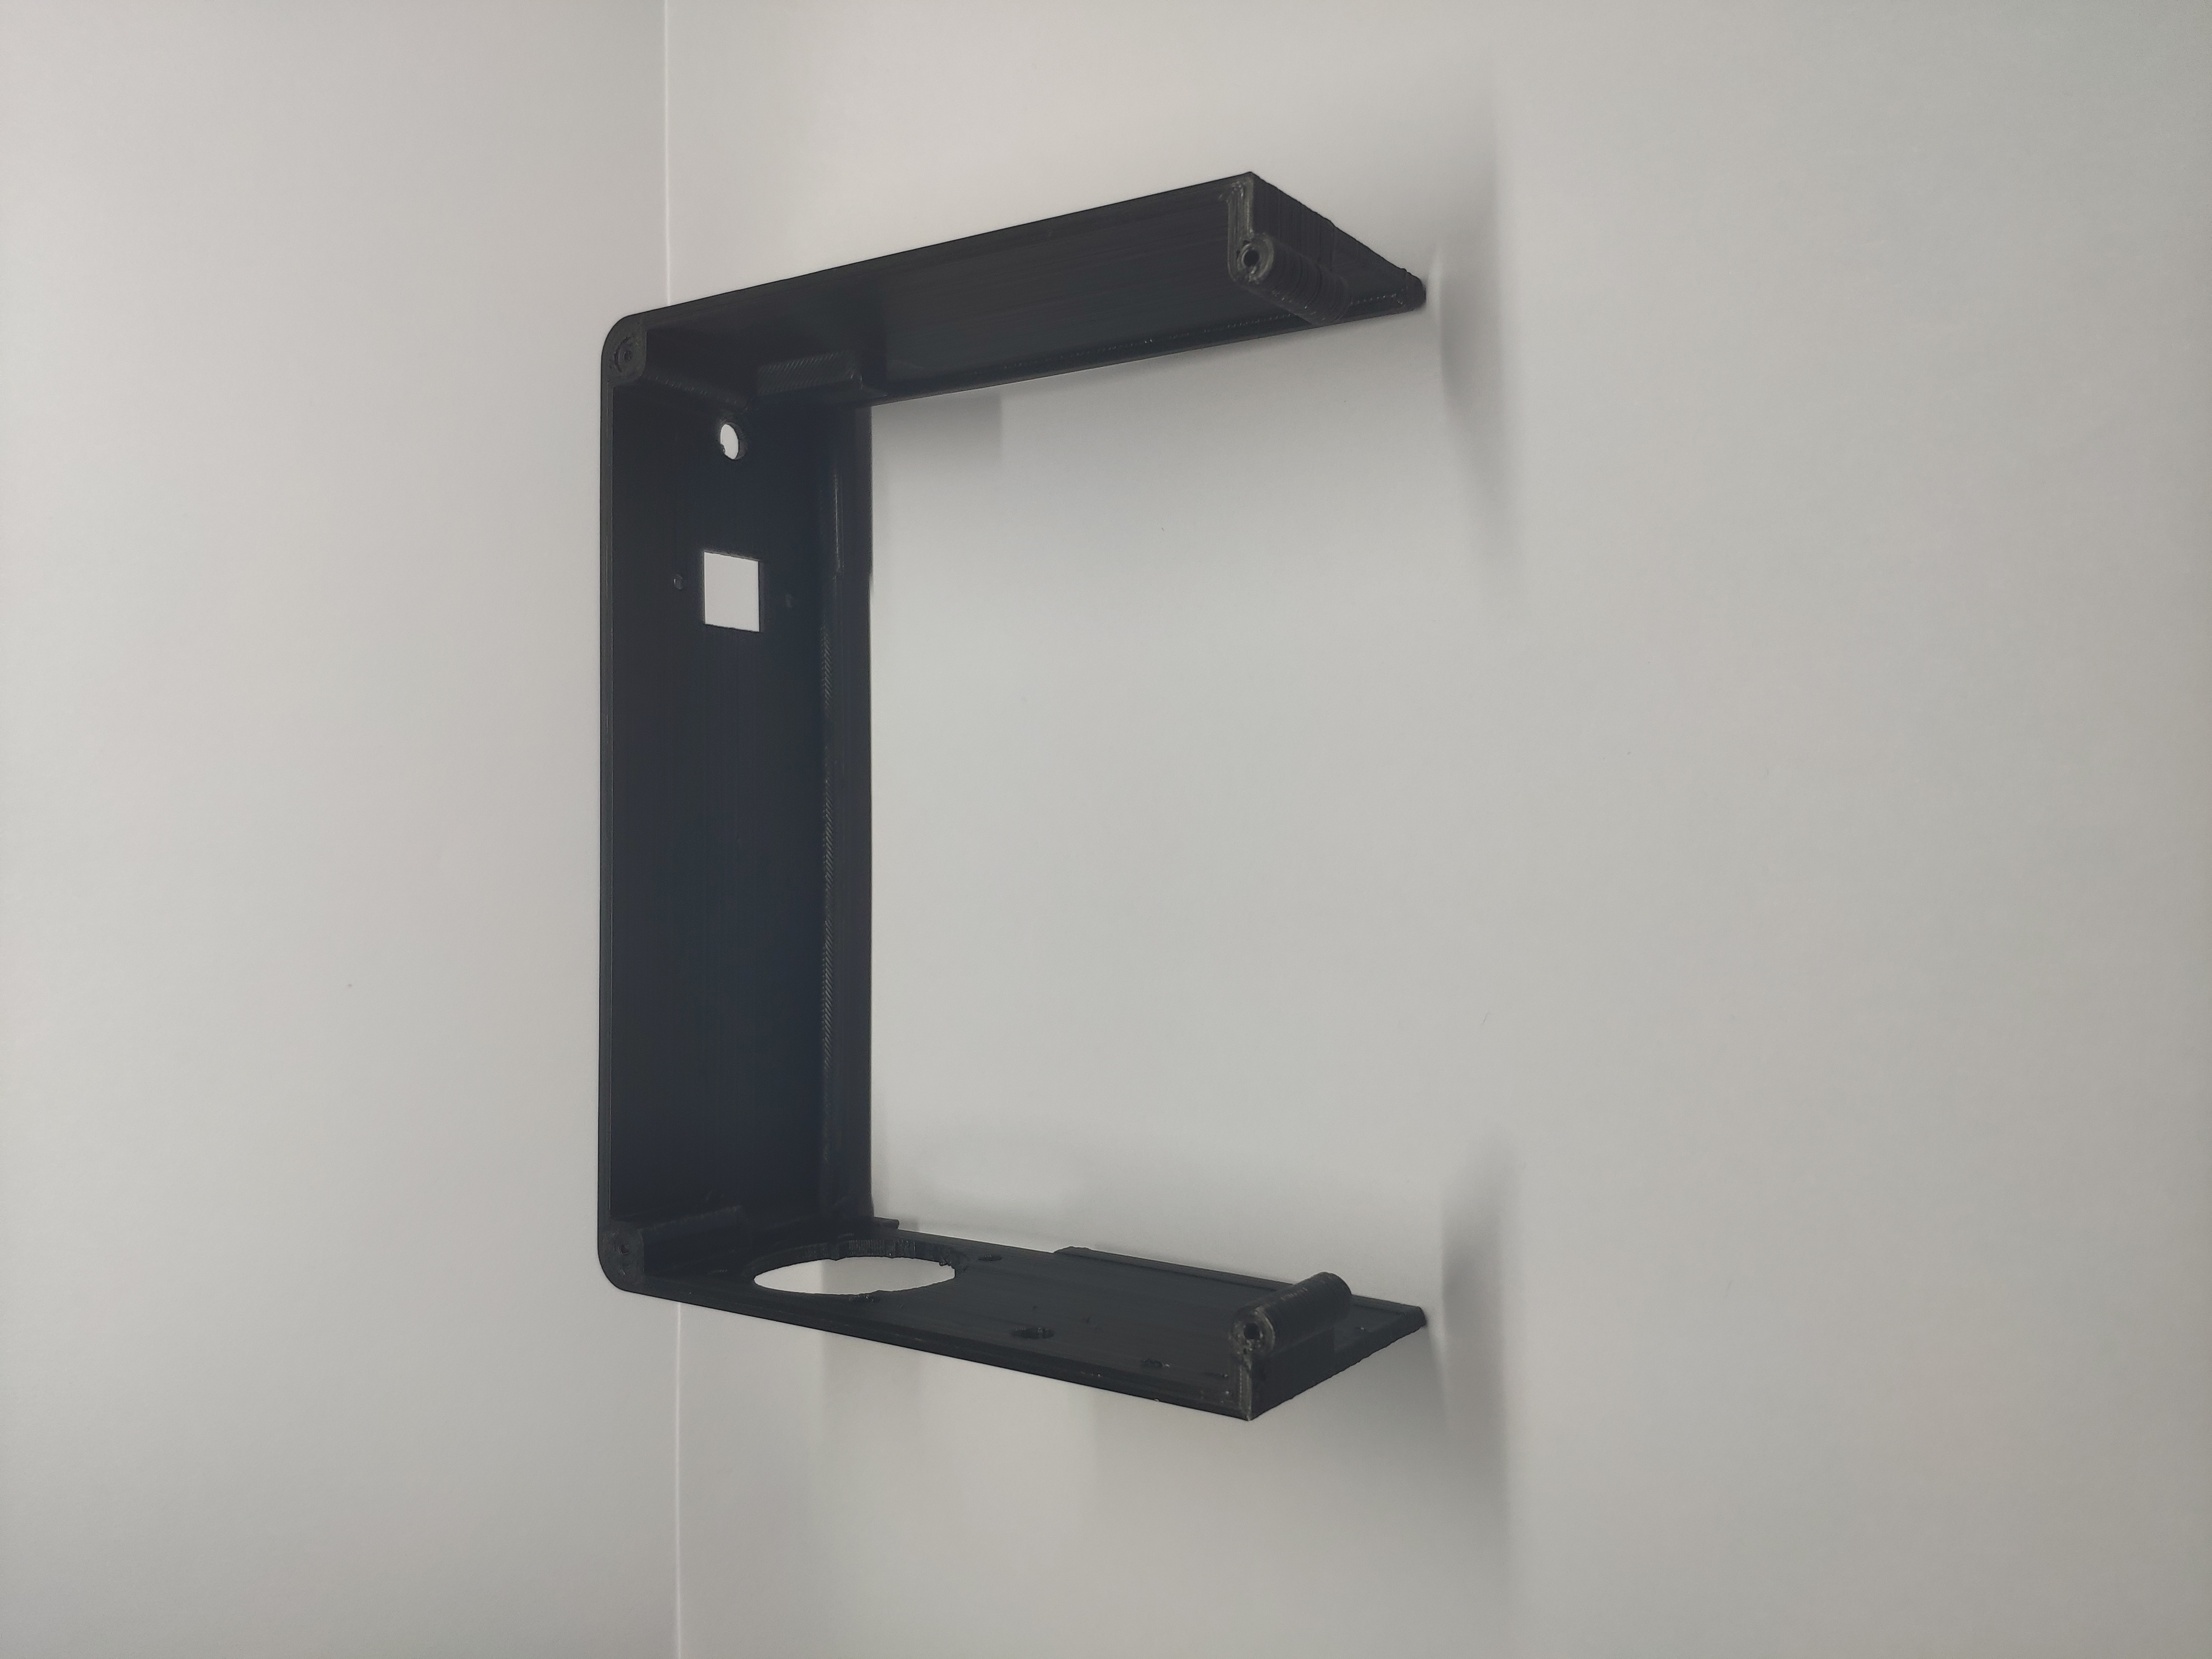
\includegraphics[width=1\linewidth,angle=270]{img/gehauese_rechts.jpg}
		\caption[Rechte Seite]{Rechte Seite}
		\label{printet_parts_right}
	\end{subfigure}
	\caption[Ausgedruckte Teile des Gehäuses]{Ausgedruckte Teile des Gehäuses}
	\label{fig:printet_parts}
\end{figure}
\par
\begin{figure}[h!tb]
	\begin{subfigure}[b]{0.5\linewidth}
		\centering
		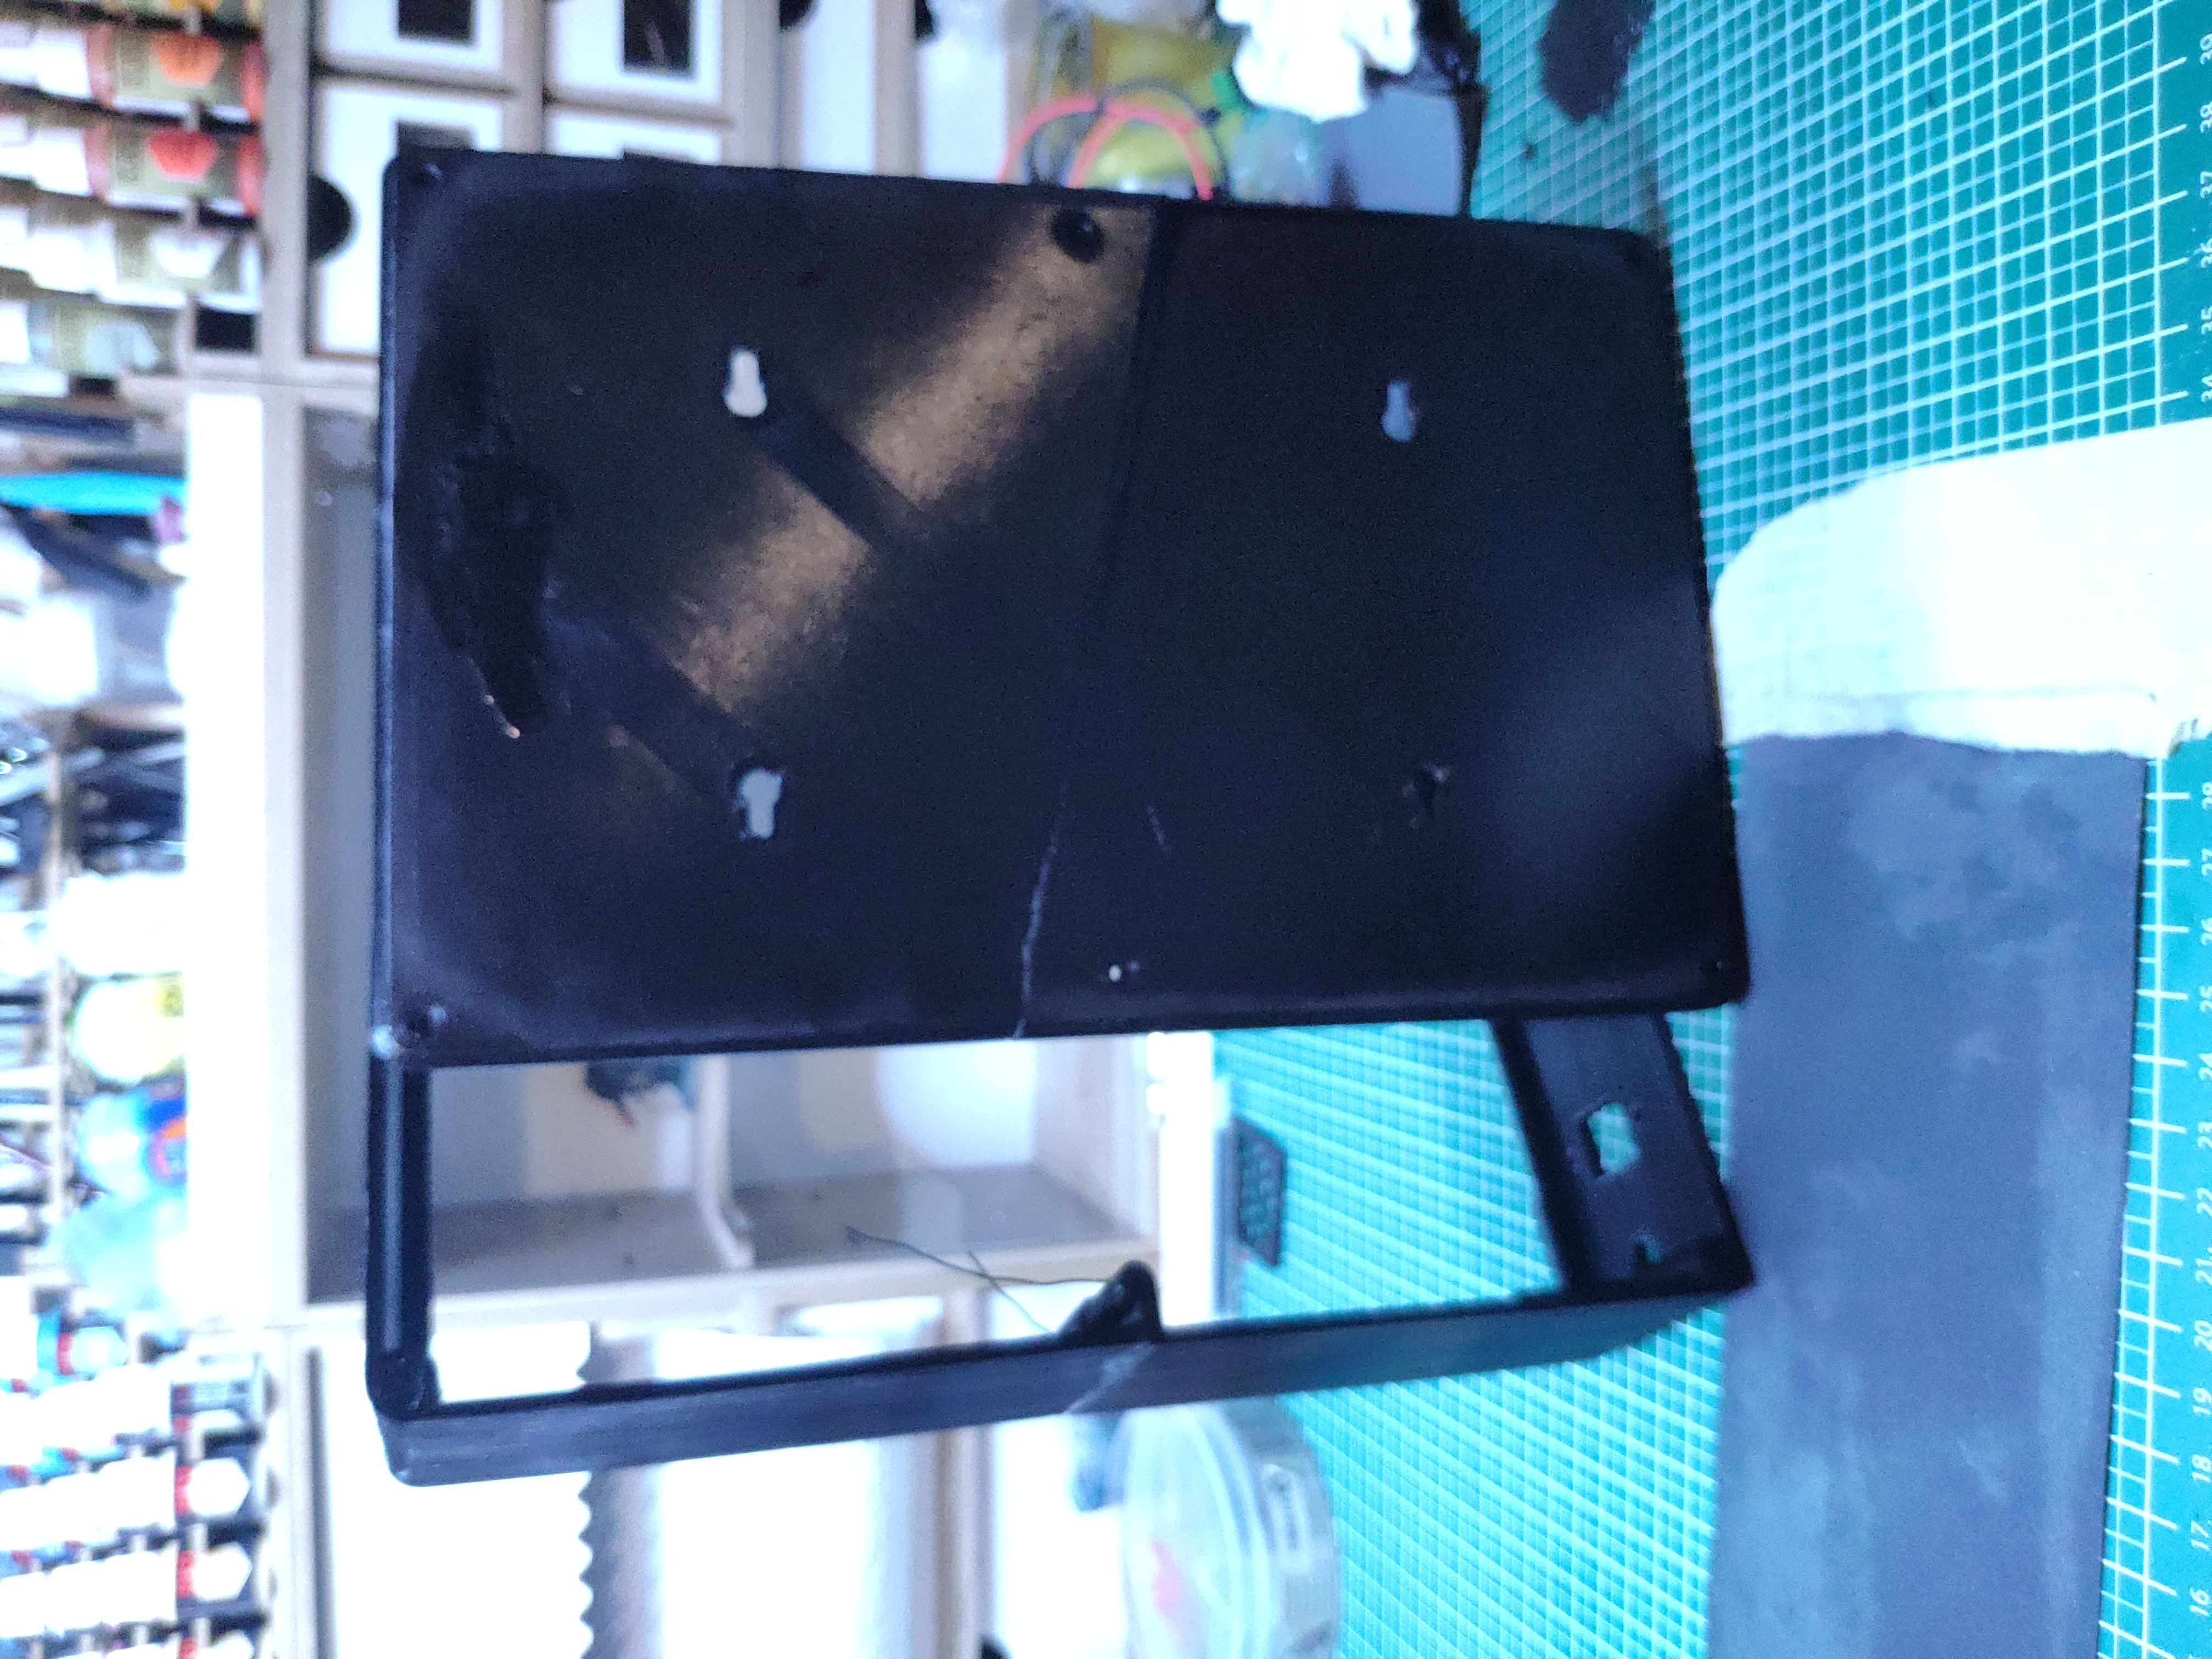
\includegraphics[width=1\textwidth]{img/gehaeuse-verklebt.jpg}
		\caption[Verklebung des Gehäusess]{Verklebung des Gehäuses}
		\label{fig:glued_parts}
	\end{subfigure}
	\begin{subfigure}[b]{0.5\linewidth}
		\centering
		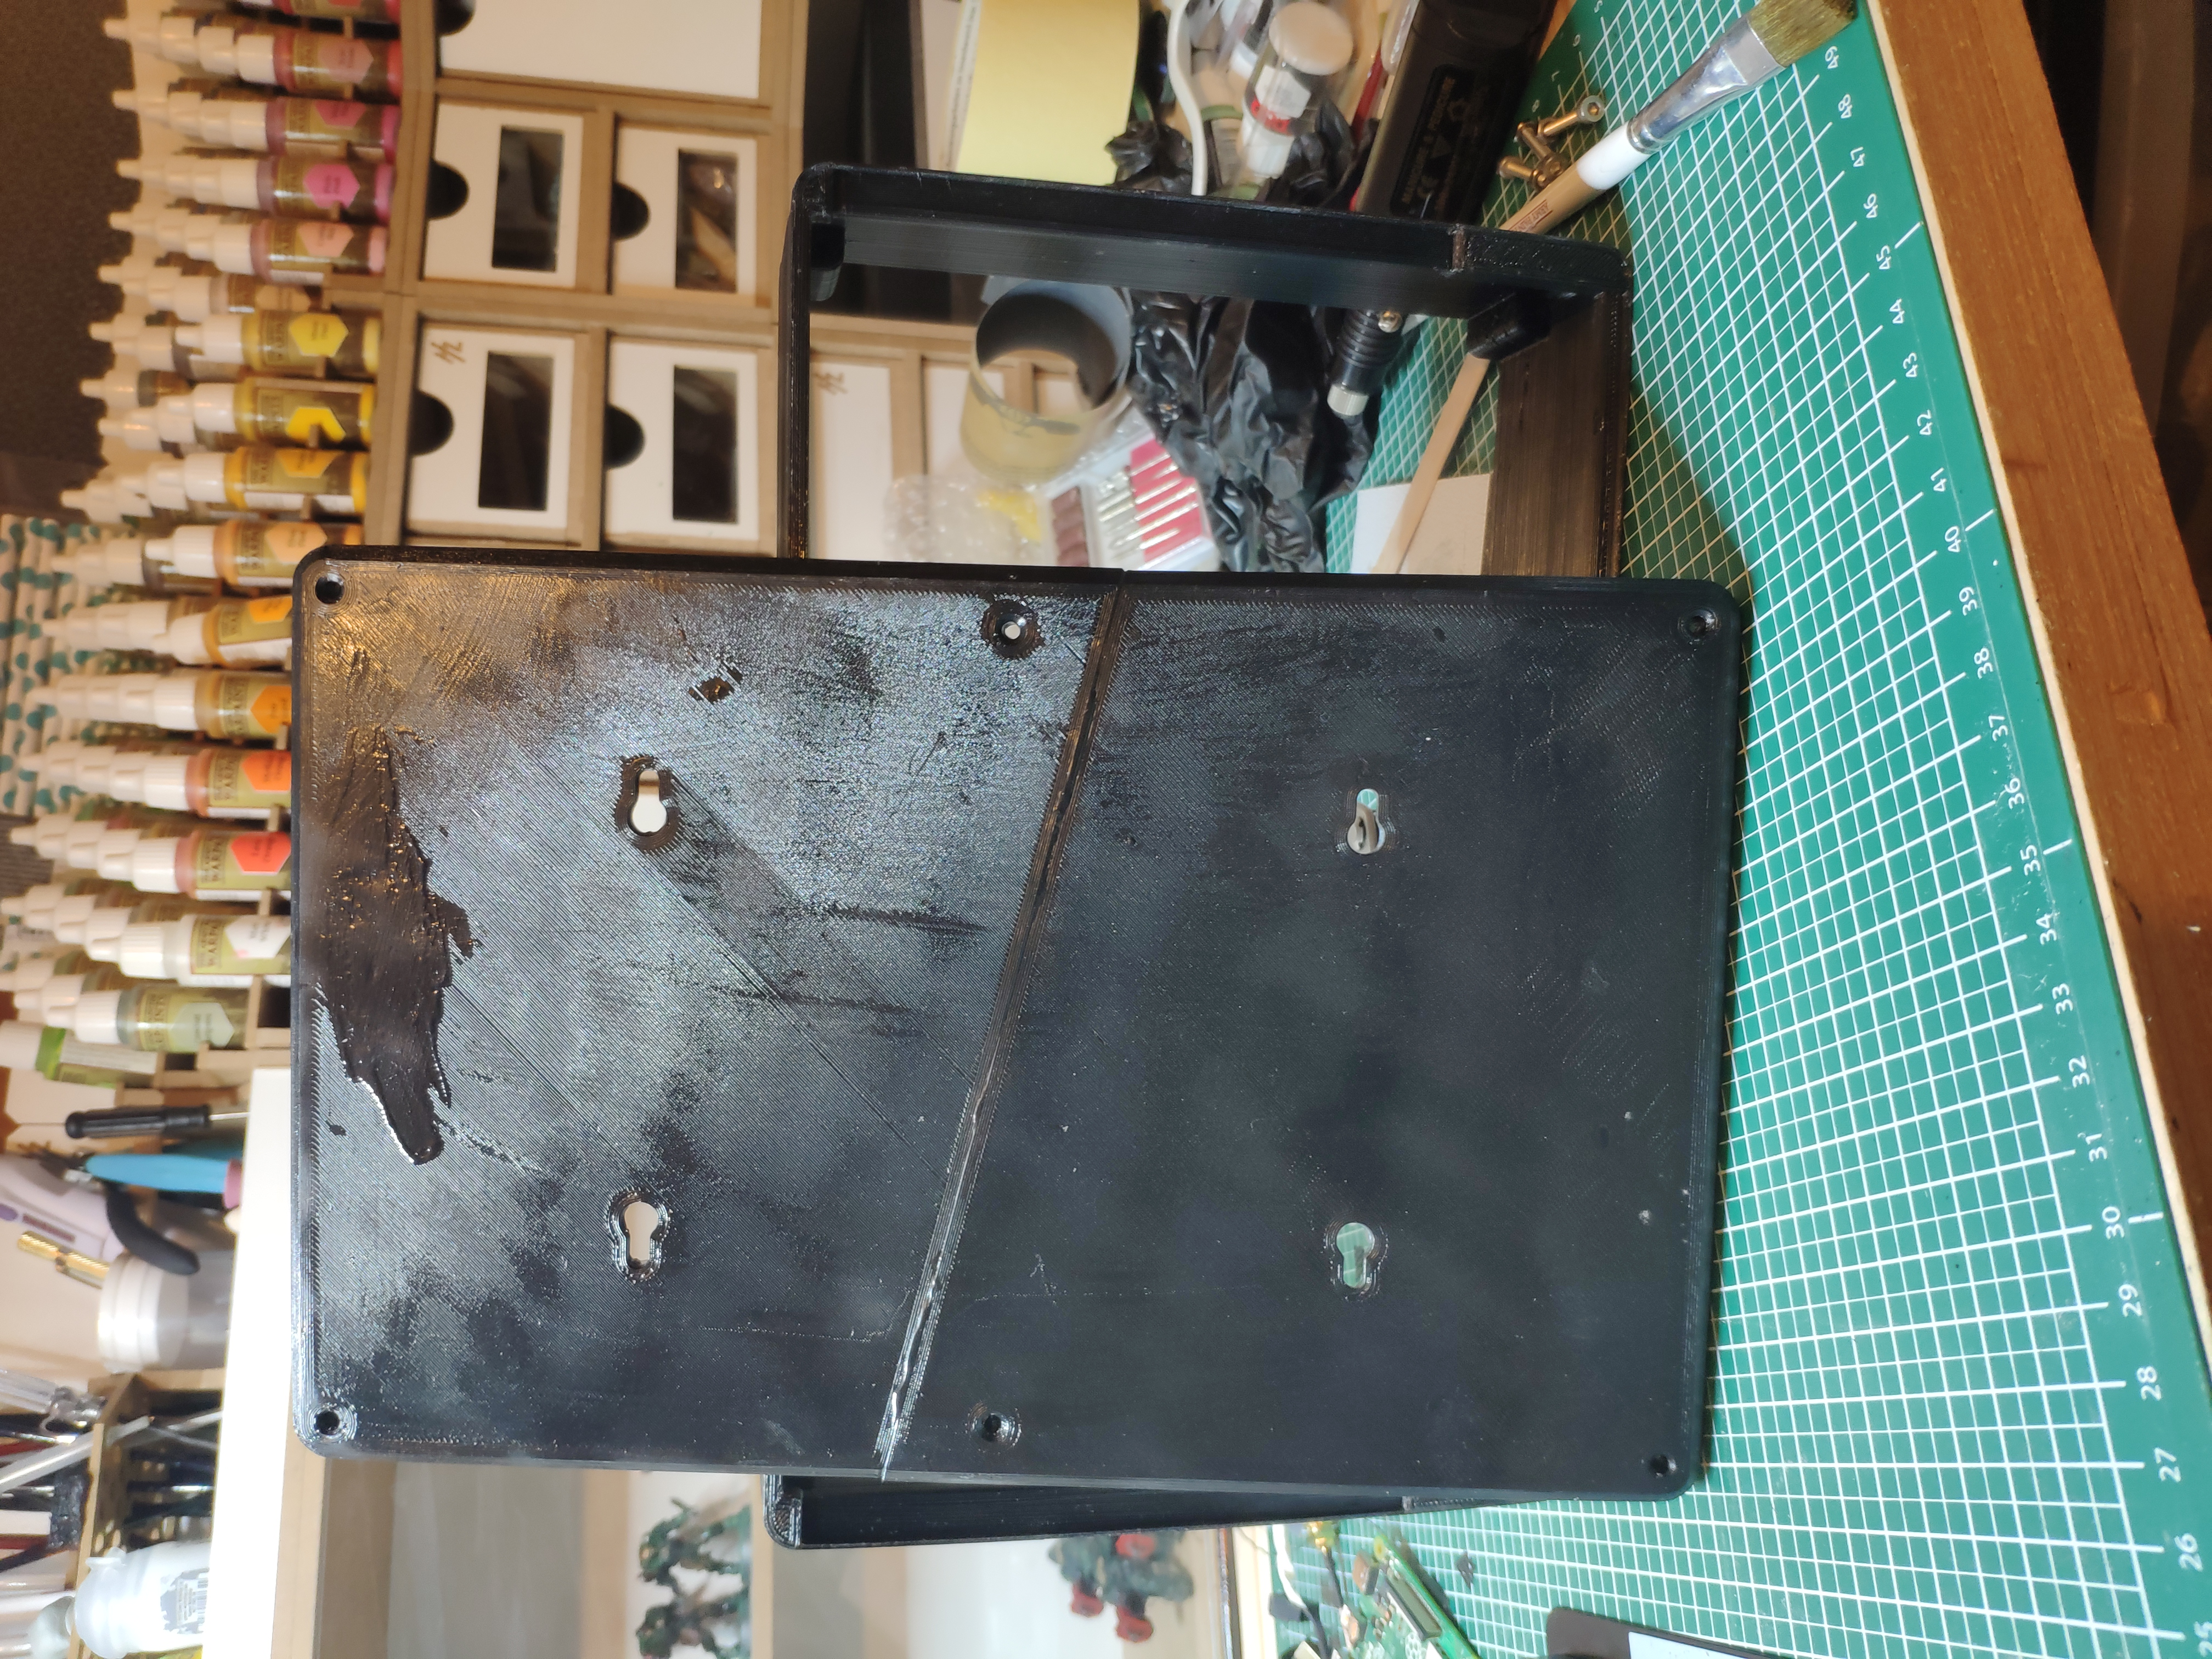
\includegraphics[width=1\textwidth]{img/gehaeuse-lakiert.jpg}
		\caption[Abgeschliffene und lackierte Teile]{Abgeschliffene und lackierte Teile}
		\label{fig:filed_and_painted_parts}
	\end{subfigure}
	\begin{subfigure}[b]{0.5\linewidth}
		\centering
		\includegraphics[width=1\textwidth]{img/geraet_front.jpg}
		\caption[Gehäuse und Bildschirm verklebt (von vorne)]{Gehäuse und Bildschirm verklebt (von vorne)}
		\label{fig:finished_case_front}
	\end{subfigure}
	\begin{subfigure}[b]{0.5\linewidth}
		\centering
		\includegraphics[width=1\textwidth]{img/geraet_rueck.jpg}
		\caption[Gehäuse und Bildschirm verklebt (von hinten)]{Gehäuse und Bildschirm verklebt (von hinten)}
		\label{fig:finished_case_back}
	\end{subfigure}
	\caption[Fertigung des Gehäuses]{Fertigung des Gehäuses}
	\label{fig:creating-case}
\end{figure}\par
\noindent Laut Ultimaker CURA beträgt die Gesamtdruckdauer des Gehäuses 36 Stunden 36 Minuten und verbraucht insgesamt 423 Gramm des verwendeten Filaments (dasFilament PETG Schwarz). 
Damit belaufen sich die Materialkosten des Gehäuses auf 11,61\euro{}.\par
\noindent Bei der Herstellung kam es aber zu einem Problem, dass die Stützstrukturen den Druck am Lüftereinlass an den Seitenwänden gestört habem was dazu führte, dass das Lüftergitter an der  linken Seitenwand (vgl. \ref{printet_parts_left}) nicht richtig gedruckt wurde.


% Raspberry Pi HAT
\subsection{Erstellung des RPi-HATs}
% Dokumentation des Testaufbaus
\subsection{Präsentationsaufbau}\label{hw_testaufbau}
\begin{figure}[H]
    \includegraphics[width=1\textwidth]{img/placeholder.png}
    \caption[Präsentationsaufbau]{Präsentationsaufbau}
    \label{fig:praesentationsaufbau}
\end{figure}
Um unsere Technikerarbeit präsentieren zu können, haben wir einen Präsentationsaufbau aus XXX gebaut (vgl. Abb. \ref{fig:praesentationsaufbau}: \nameref{fig:praesentationsaufbau}).
Dieser ist neben der Smart Home Zentrale auch mit einem Heimrouter und einer Zigbee-fähigen Glübirne ausgestattet.
Zusätzlich haben wir im Netz des Heimrouters ein Tablet eingebunden, welches ebenfalls auf die Weboberfläche der Smart Home Zentrale zugreifen kann (vgl. Abb. \ref{fig:praesentationsaufbau_diagramm}: \nameref{fig:praesentationsaufbau_diagramm}).
\begin{figure}[H]
    \includegraphics[width=1\textwidth]{img/placeholder.png}
    \caption[Plandiagramm des Aufbaus]{Plandiagramm des Aufbaus}
    \label{fig:praesentationsaufbau_diagramm}
\end{figure}
\newpage
	% Software
	\section{Software}
% Überblick
\subsection{Überblick}\label{sw_ueberblick}
Auf der Softwareseite dient Raspberry Pi OS\footnote{Raspberry Pi OS with Desktop, Kernel Version 5.4} als Basis für die Smart Home Zentrale.
Darauf laufen die gewählten Softwarelösungen
\begin{itemize}
\item Home Assistant Supervised (Web Oberfläche und Verwaltung)
\item Mosquitto Broker (MQTT Broker)
\item Zigbee2mqtt (Zigbee-Schnittstelle)
\end{itemize}
\noindent Zur Installation der einzelnen Komponenten und für die Vorkonfiguration des Systems haben wir ein bash-Skript (vgl. \ref{ah_skript}) erstellt, dass das System entsprechend vorbereitet und die einzelnen Komponenten installiert.
% MQTT-Broker
\subsection{Mosquitto Broker}\label{sw_mqtt-broker}
Als erste wichtige Erweiterung benötigen wir für unseren Home Assistant einen MQTT Broker. 
Da wir eine Supervised Version des Home Assistant auf unserem Pi vewenden, nutzen wir für die Installation den Supervisor Add-on Shop von Home Assistant (vgl. Abb.  \ref{fig:ha11}: \nameref{fig:ha11}).\\
\noindent Hier wählen wir den Mosquitto Broker zur Installation aus (vgl. Abb. \ref{fig:ha12}: \nameref{fig:ha12}). 
Um den Mosquitto Broker zu aktivieren, navigieren wir über den Menüpunkt ,,Einstellungen'' zum Punkt ,,Integrationen'' und suchen dort nach MQTT. 
Wir aktivieren die Verknüpfung von Home Assistant und Mosquitto Broker, indem wir die Schaltfläche ,,Suche aktivieren'' klicken.
Nach Durchführung dieser Schritte ist der Mosquitto Broker aktiv.
\begin{figure}[H]
    \begin{subfigure}{.5\linewidth}
        \includegraphics[width=1\textwidth]{img/HA6.png}
        \caption{Supervisor Dashboard}
        \label{fig:ha5}
    \end{subfigure}
    \begin{subfigure}{.5\linewidth}
        \includegraphics[width=1\textwidth]{img/HA7.png}
        \caption{Supervisor Add-on Shop}
        \label{fig:ha6}
    \end{subfigure}
    \begin{subfigure}{.5\linewidth}
        \includegraphics[width=1\textwidth]{img/HA8.png}
        \caption{MQTT add-on seite}
        \label{fig:ha7}
    \end{subfigure}
    \begin{subfigure}{.5\linewidth}
        \includegraphics[width=1\textwidth]{img/HA9.png}
        \caption{Einstellungen}
        \label{fig:ha8}
    \end{subfigure}
    \begin{subfigure}{.5\linewidth}
        \includegraphics[width=1\textwidth]{img/HA12.png}
        \caption{Startseite Integrationen }
        \label{fig:ha11}
    \end{subfigure}
    \begin{subfigure}{.5\linewidth}
        \includegraphics[width=1\textwidth]{img/HA13.png}
        \caption{Suchfunktion Integrationen }
        \label{fig:ha12}
    \end{subfigure}
    \begin{subfigure}{.5\linewidth}
        \includegraphics[width=1\textwidth]{img/HA14.png}
        \caption{Suche nach MQTT }
        \label{fig:ha13}
    \end{subfigure}
\end{figure}

%\begin{figure}[H]
%    \includegraphics[width=1\textwidth]{img/HA6.png}
%    \caption{Supervisor Dashboard}
%    \label{fig:ha5}
%\end{figure}
%\begin{figure}[H]
%    \includegraphics[width=1\textwidth]{img/HA7.png}
%    \caption{Supervisor Add-on Shop}
%    \label{fig:ha6}
%\end{figure}
%\begin{figure}[H]
%    \includegraphics[width=1\textwidth]{img/HA8.png}
%    \caption{MQTT add-on seite }
%    \label{fig:ha7}
%\end{figure}
%\begin{figure}[H]
%    \includegraphics[width=1\textwidth]{img/HA9.png}
%    \caption{Einstellungen}
%    \label{fig:ha8}
%\end{figure}
%\begin{figure}[H]
%    \includegraphics[width=1\textwidth]{img/HA10.png}
%    \caption{Benuterverwaltung}
%    \label{fig:ha9}
%\end{figure}
%\begin{figure}[H]
%    \includegraphics[width=1\textwidth]{img/HA11.png}
%    \caption{Benutzer MQTT anlegen }
%    \label{fig:ha10}
%\end{figure}
% HomeAssistant
\subsection{HomeAssistant}\label{sw_hassio}
% MyCroft
\subsection{MyCroft}\label{sw_mycroft}
% HAT-Programm
%\subsection{HAT-Programm}\label{sw_hat}
\newpage
	% Epilog & Fazit
	\section{Epilog \& Fazit}
% Latex vs. Word
\subsubsection{\LaTeX vs Word}\label{fz_LatexVsWord}
Danke Herr Kohler. 
Ihre fast 2 Jahre langes Gejammer über WYSIWYG-Dokumenteneditoren haben dazu geführt, dass wir uns in den letzten Zügen der Dokumentation dazu entschlossen haben, OHNE JEGLICHE VORERFAHRUNG diese in \LaTeX zu schreiben. 
Ich hoffe, Sie sind stolz auf das Monster, dass Sie geschaffen haben...
\newpage	
	% Quellen
	\section{Quellen}
% Dokumentationsquellen
\subsection{Dokumentationsquellen}
Quellen für Verweise, die in Fußnoten innerhalb dieser Dokumentation erwähnt wurden:
\begin{itemize}
 		\item Li (2017): Was ist ein Smart-Home-Hub? Alles über die intelligente Zentrale\\ {\url{https://www.otto.de/updated/ratgeber/erklaert-was-ist-ein-smart-home-hub-80634/}}
 		\item Robert (2019): Antwort auf Creality Ender 3 printer power consumption? - 3dprinting Stack Exchange\\ {\url{https://3dprinting.stackexchange.com/questions/8616/creality-ender-3-printer-power-consumption#8623/}}
\end{itemize}
Quellen, die für die Herstellung dieser Dokumentation genutzt wurden:
\begin{itemize}
	\item Menmiloud Mohammed: \LaTeX -Tutorial.com\\{\url{https://latex-tutorial.com/}}
	\item Overleaf: \LaTeX -Guides\\{\url{https://www.overleaf.com/learn}}
\end{itemize}
% verwendete Software
\subsection{Verwendete Software}\label{qu_software}
\begin{table}[H]
\begin{tabularx}{\textwidth}{|p{5cm}|p{6cm}|p{3.2cm}|}
 	\hline 
 	\textbf{Software} & \textbf{Verwendung} & \textbf{Version} \\ 
 	\hline 
 	Raspberry Pi OS & Betriebssystem und Oberfläche für Hardware & 5.4 \\ 
 	\hline 
 	Home Assistant & Betriebssystem und Oberfläche für Smart Home & 5.12 \\ 
 	\hline
 	Mosquitto broker & Broker für den MQTT nachrichten Standart & 5.1.1 \\ 
 	\hline
 	Zigbee2MQTT & Anbindung von Zigbee an MQTT & 1.18.1-2 \\ 
 	\hline
 	KiCad EDA & Erstellung von Schaltplan und Gerber-Datei des Hats & 5.1.8 \\ 
 	\hline 
 	TexMaker & Erstellung der Dokumentation & 5.0.4 \\ 
 	\hline
 	\url{overleaf.com } & Gemeinsame Erstellung der Dokumentation & Web \\
 	\hline
 	Fusion360 & Erstellung von Gehäusemodell & 2.0.9849 \\ 
 	\hline
 	CURA & Erstellung von G-Code für 3D-Drucker & 4.7 \\ 
 	\hline
 	GanttProject & Erstellung von Gantt-Diagrammen & 3.0.3 \\ 
 	\hline
 	Autodesk Meshmixer & Vorschau-Render der STL-Dateien & 3.5.474 \\
 	\hline
 	paint.net & Bildmanipulation & 4.2.15\\
 	\hline
 	Win32 Disk Imager & Erstellung der Image aus den Micro-SD-Karten & 1.0 \\
 	\hline
 	7Zip & Komprimieren der Images & 19.00\\
 	\hline
 	\url{shellcheck.net/} & Überprüfung von Bash-Skripten & Web \\
 	\hline
 	\url{deepl.com/translator} & Übersetzungssoftware & Web \\
 	\hline
\end{tabularx} 
\caption{Verwendete Software}
\label{tab:qu_software}
\end{table}
% verwendete Hardware
\subsection{Verwendete Hardware}
\begin{tabular}{|l|l|l|}
 	\hline
 	\textbf{Hardware} & \textbf{Verwendung} & \textbf{Version} \\
 	\hline
 	Raspberry Pi & Hauptplatine für die  & Version 4B (8GB)\\
 	 & Smart Home Zentrale &\\
 	\hline
 	CC2531 Zigbee USB & USB-Stick mit ZigBee-Chip & Rev 2.4\\
 	Stick mit Firmware& & \\
 	\hline
 	Sunfounder 10.1  & Bildschirm und Input für & Unbekannt\\
 	Touch Screen & die Smart Home Zentrale & \\
 	 \hline
 \end{tabular}
\newpage
	% Anhang
 	\section{Anhang}
% Lastenheft
\subsection{Lastenheft}
\includegraphics*[width=1\textwidth, page=1]{pdf/lastenheft.pdf}
\newpage
\includegraphics*[width=1\textwidth, page=2]{pdf/lastenheft.pdf}
\newpage
% Gehäusezeichnungen/ -pläne
\subsection{Gehäuse-Zeichunungen}\label{ah_gehaeuse}
\includegraphics*[width=1\textwidth,page=1]{pdf/gehäuse_zeichnung_fußabdruck_v1.pdf}
\label{fig:case_footprint}
Erster Versuch der Zeichnung des Fußabdruckes des Gehäuses
\newpage
\includegraphics*[width=1\textwidth,page=1]{pdf/gehäuse_zeichnung_fußabdruck_final.pdf}
\label{fig:case_footprint_final}
Finale Version der Zeichnung des Fußabdruckes des Gehäuses
\newpage
\includegraphics*[width=1\textwidth,page=1]{pdf/gehäuse_wand_links.pdf}
Linker Teil des Gehäuses
\label{fig:case_left}
\newpage
\includegraphics*[width=1\textwidth,page=1]{pdf/gehäuse_wand_rechts.pdf}
Rechter Teil des Gehäuses
\label{fig:case_right}
\newpage
\includegraphics*[width=1\textwidth,page=1]{pdf/gehäuse_deckel.pdf}
Ein Teil des Gehäusesdeckels
\label{fig:case_back}
\newpage
% HAT-Doku
\subsection{Raspberry Pi HAT E-Schema}
\includegraphics*[width=1.4\textwidth,angle=270]{pdf/rpi-hat-eschema.pdf}
\newpage
% Hardware-Dokus
\subsection{Hardware-Dokumentationen}
Durch den Umfang der einzelnen Dokumentationen hier nur eine Auflistung der Dokumentationen mit dem Link zu den PDF im GIT-Projekt bzw. den Herstellerseiten.
\begin{itemize}
 	\item Raspberry Pi:\\ {\url{https://www.raspberrypi.org/documentation/hardware/raspberrypi/bcm2711/rpi_DATA_2711_1p0.pdf}}
 	\item MiFare MFRC522:\\ {\url{https://www.nxp.com/docs/en/data-sheet/MFRC522.pdf}}
 	\item CC2531 ZigBee SoC:\\ {\url{https://www.ti.com/lit/ds/symlink/cc2531.pdf}}
 	\item ATmega128RFA1-ZU:\\ {\url{https://ww1.microchip.com/downloads/en/DeviceDoc/Atmel-8266-MCU_Wireless-ATmega128RFA1_Datasheet.pdf}}
\end{itemize}
\newpage

 	% Abbildungsverzeichnis
 	\listoffigures
\end{document}
